%%%%%%%%%%%%%%%%%%%%%%%%%%%%%%%%%%%%%%%%%%%%%%%%%%%
%% Document Class

\documentclass[review,11pt]{elsarticle}
%\documentclass[final,5p,times,twocolumn]{elsarticle}

\journal{Fire Safety Journal}

%%%%%%%%%%%%%%%%%%%%%%%%%%%%%%%%%%%%%%%%%%%%%%%%%%%
%% Bibliography

\bibliographystyle{elsarticle-num}
\biboptions{comma,square,numbers,sort&compress}

%%%%%%%%%%%%%%%%%%%%%%%%%%%%%%%%%%%%%%%%%%%%%%%%%%%
%% Packages

\usepackage{lineno}
\usepackage{booktabs}
\usepackage{graphicx}
\usepackage{amsmath}
\usepackage{amssymb}

%\usepackage{xr-hyper}
\usepackage[pdftex,
        colorlinks=true,
        urlcolor=linkblue,     % \href{...}{...} external (URL)
        citecolor=linkred,     % citation number colors
        linkcolor=linknavy,    % \ref{...} and \pageref{...}
        pdfproducer={pdflatex},
        pagebackref,
        pdfpagemode=UseNone,
        bookmarksopen=true,
        plainpages=false,
        verbose]{hyperref}

\usepackage{geometry}
\geometry{letterpaper, margin=1in}

\usepackage{lipsum}

\usepackage[nooneline]{subfigure}
%\subfigtopskip = 0cm
\subfigcapskip = -5mm
\subfigcapmargin = -3.5mm
%\subfigcaptopadj = 7cm
%\subfigbottomskip = 0cm
%\subfiglabelskip = -1cm

\usepackage{hyperref}
\hypersetup{colorlinks=true,linkcolor=blue}

\usepackage{caption}

\renewcommand*{\today}{July 11, 2018}

%%%%%%%%%%%%%%%%%%%%%%%%%%%%%%%%%%%%%%%%%%%%%%%%%%%

\begin{document}

\begin{frontmatter}

\title{Proceedings of the First Workshop Organized by the IAFSS Working Group on Measurement and Computation of Fire Phenomena (MaCFP)}


\author[label:Sandia]{A.~Brown}
\author[label:NIST]{M.~Bruns}
\author[label:UMD]{M.~Gollner}
\author[label:Sandia]{J.~Hewson}
\author[label:UMD]{A.~Marshall}
\author[label:NIST]{R.~McDermott}
\author[label:Ghent]{G.~Maragkos}
\author[label:Ghent]{B.~Merci}
\author[label:Poitiers]{T.~Rogaume}
\author[label:UMD]{S.~Stoliarov}
\author[label:UMD]{J.~Torero}
\author[label:UMD]{A.~Trouv\'{e}\corref{cor1}}
\ead{atrouve@umd.edu}
\author[label:FM]{Y.~Wang}
\author[label:Waterloo]{E.~Weckman}

\address[label:Sandia]{Fire Science and Technology Department, Sandia National Laboratories, Albuquerque,~NM~87185,~USA}
\address[label:NIST]{Fire Research Division, National Institute of Standards and Technology, Gaithersburg,~MD~20899,~USA}
\address[label:UMD]{Department of Fire Protection Engineering, University of Maryland, College~Park,~MD~20742,~USA}
\address[label:Ghent]{Department of Flow, Heat and Combustion Mechanics, Ghent University-UGent,~B-9000~Ghent,~Belgium}
\address[label:Poitiers]{Institut Pprime (UPR 3346 CNRS), Universit\'{e} de Poitiers, Isae-ENSMA,~86961~Futuroscope~Chasseneuil~Cedex,~France}
\address[label:FM]{FM Global, Research Division, Norwood,~MA~02062,~USA}
\address[label:Waterloo]{Department of Mechanical and Mechatronics Engineering, University of Waterloo, Waterloo,~Ontario,~N2L~3G1,~Canada}

\cortext[cor1]{Corresponding author}

\begin{abstract}

This paper provides a report of the discussions held at the first workshop on Measurement and Computation of Fire Phenomena (MaCFP) on June 10-11 2017. The first MaCFP workshop was both a technical meeting for the gas phase subgroup and a planning meeting for the condensed phase subgroup. The gas phase subgroup reported on a first suite of experimental-computational comparisons corresponding to an initial list of target experiments. The initial list of target experiments identifies a series of benchmark configurations with databases deemed suitable for validation of fire models  based on a Computational Fluid Dynamics approach. The simulations presented at the first MaCFP workshop feature fine grid resolution at the millimeter- or centimeter-scale: these simulations allow an evaluation of the performance of fire models under high-resolution conditions in which the impact of numerical errors is reduced and many of the discrepancies between experimental data and computational results may be attributed to modeling errors. The experimental-computational comparisons are archived on the MaCFP repository~\cite{MaCFP_repository}. Furthermore, the condensed phase subgroup presented a review of the main issues associated with measurements and modeling of pyrolysis phenomena. Overall, the first workshop provided an illustration of the potential of MaCFP in providing a response to the general need for greater levels of integration and coordination in fire research, and specifically to the particular needs of model validation.

\end{abstract}

\begin{keyword}
Buoyant plumes \sep Pool fires \sep Wall fires \sep Flame extinction \sep Fire modeling \sep Pyrolysis modeling \sep Large Eddy Simulation
\end{keyword}

\end{frontmatter}

\pagenumbering{arabic}
\setcounter{page}{1}
\linenumbers

% change "include" to "input" for final paper

% !TEX root = macfp_2017_gasphase.tex

\section{Introduction} \label{sec:intro}

A new initiative, endorsed and supported by the International Association for Fire Safety Science (IAFSS)~\cite{IAFSS_website}, has been launched: the ``{\it IAFSS Working Group on Measurement and Computation of Fire Phenomena}" (or the MaCFP Working Group)~\cite{MaCFP_website}. The general objective of the MaCFP Working Group is to establish a structured effort in the fire research community in order to make significant and systematic progress in fire modeling through a fundamental understanding of fire phenomena. This is to be achieved as a joint effort between experimentalists and modelers on the general topic of the experimental validation of fire models based on a Computational Fluid Dynamics (CFD) approach. The MaCFP Working Group is intended as an open, community-wide, international collaboration between fire scientists. It is also intended to become a regular series of workshops, with workshops held every two or three years. The first workshop organized by the MaCFP Working Group was held as a pre-event to the 12th IAFSS Symposium in Lund, Sweden, on June 10-11 2017~\cite{MaCFP_wks_presentations}. This paper presents a summary of the discussions and outcomes of the first MaCFP workshop.

The content and format of the first MaCFP workshop had been previously decided during a planning meeting in 2015. The planning meeting had produced a list of target experiments with databases deemed suitable for validation of CFD-based fire models. The intent was to make sure that the first workshop would go beyond the level of general discussions and would include presentations of a first suite of experimental-computational comparisons corresponding to an initial list of relevant experiments. The list of target experiments and a call for participation in the first workshop were broadly advertised to the international fire research community through letters to the editors of {\it Fire Safety Journal}~\cite{MaCFP_FSJ} and {\it Fire Technology}~\cite{MaCFP_FT} as well as through emails to the IAFSS membership.

While early discussions of the MaCFP Working Group had focused on gas phase phenomena (primarily flow and combustion phenomena), discussions were started in 2016 to expand the scope of MaCFP to include a subgroup dedicated to the modeling of pyrolysis phenomena. This led to a re-structuring of MaCFP into two subgroups: the (original) ``{\it gas phase subgroup}" and the (new) ``{\it condensed phase subgroup}". Thus, in addition to being a first technical meeting for the gas phase subgroup, the June-2017 MaCFP workshop also served as a planning meeting for the condensed phase subgroup. The planning meeting portion of the workshop included a review of the main issues associated with pyrolysis measurements and modeling for fire applications and a discussion of future priorities for the condensed phase subgroup.

The technical meeting portion of the workshop provided a first demonstration of current activities of the MaCFP Working Group as well as an illustration of their potential impact. The initial list of target experiments identified by the gas phase subgroup corresponds to basic configurations (also called building blocks) featuring carefully-controlled conditions and quality instrumentation and diagnostics. They also correspond to experiments with open, easily-accessible databases. In what is considered as a first intermediate step, the list has a limited scope and only includes simple turbulent buoyant plumes and simple flames (in most cases, the flames are non-sooting or only weakly-sooting), supplied with gaseous or liquid fuel, and featuring open burn conditions; the case of strongly sooting and smoking flames, fueled by solid flammable materials, and featuring compartment effects is outside the scope of the first MaCFP workshop and will be considered in future editions.

The initial list of MaCFP target experiments includes five categories:
\begin{itemize}
\item (Case 1) Turbulent buoyant plumes: this category corresponds to open plumes and is represented by a helium plume experiment conducted at Sandia National Laboratories (Sandia)~\cite{Case1_EXP}.
\item (Case 2) Turbulent pool fires with gaseous fuel: this category corresponds to open flames with a prescribed fuel flow rate and is represented by a series of natural gas flame experiments conducted at the National Institute of Standards and Technology (NIST)~\cite{Case2a_EXP} (and referred to in the following as the NIST McCaffrey natural gas flame experiment) and by a series of methane and hydrogen fire experiments conducted at Sandia National Laboratories (Sandia)~\cite{Case2b_EXP_CH4,Case2b_EXP_H2}.
\item (Case 3) Turbulent pool fires with liquid fuel: this category corresponds to open flames with a thermal-feedback-driven fuel flow rate and is represented by a methanol pool fire experiment conducted at the University of Waterloo (UW)~\cite{Case3_EXP_1,Case3_EXP_2}.
\item (Case 4) Turbulent wall fires: this category corresponds to boundary layer flames with a prescribed fuel flow rate and is represented by a series of vertical wall flame experiments, fueled by methane, ethane, ethylene or propylene, and conducted at FM Global~\cite{Case4_EXP_1,Case4_EXP_2}.
\item (Case 5) Flame extinction: this category corresponds to flames driven to extinction conditions and is represented by a series of methane and propane line flame experiments conducted at the University of Maryland (UMD)~\cite{Case5_EXP_1,Case5_EXP_2,Case5_EXP_3}.
\end{itemize}

Note that the experimental databases corresponding to Cases 1-5 are hosted on the MaCFP repository~\cite{MaCFP_repository} with open access so that the data are available to the fire research community as reference data for future experimental and/or computational studies.

Seven groups submitted computational results for comparisons with experimental data and for discussions at the first MaCFP workshop: FM Global (USA); Ghent University (UGent, Belgium); the Institut de Radioprotection et de S\^uret\'e Nucl\'eaire (IRSN, France); the National Institute of Standards and Technology (NIST, USA) teamed up with the VTT Technical Research Centre of Finland (VTT, Finland); Sandia National Laboratories (SNL, USA); University of Cantabria (UCantabria, Spain); and University of Maryland (UMD, USA). These groups used one of the following four CFD solvers:

\begin{itemize}
\item FDS (Fire Dynamics Simulator) developed by NIST in collaboration with VTT~\cite{FDS};
\item FireFOAM based on OpenFOAM~\cite{OpenFOAM} and developed by FM Global~\cite{FireFOAM};
\item ISIS developed by IRSN~\cite{ISIS};
\item SIERRA/Fuego developed by SNL~\cite{SIERRA/Fuego}.
\end{itemize}

These solvers are representative of current fire modeling capabilities available for research-level and/or engineering-level projects.

The paper is structured as follows. Section~\ref{sec:GPS_session} describes the main outcomes of the technical meeting held by the gas phase subgroup of the MaCFP Working Group. Section~\ref{sec:cfd_review} gives a brief description of the different concepts used in quality control of CFD models and a review of the computational challenges found in model validation (the focus of MaCFP). Sections~\ref{sec:buoyant_plumes}-\ref{sec:flame_extinction} present a summary of the experimental-computational comparisons performed for Cases 1-5, respectively. Section~\ref{sec:plans} presents a conclusion and a description of future plans for the gas phase subgroup. Section~\ref{sec:CPS_session} presents a review of the discussions held during the planning meeting of the condensed phase subgroup of the MaCFP Working Group. Section~\ref{sec:CPS_session_1} gives a brief description of the objectives of the subgroup. Section~\ref{sec:CPS_session_2} presents a summary of the invited presentations and follow-up discussion that took place at the workshop. Section~\ref{sec:CPS_session_3} presents a conclusion and a description of future plans for the condensed phase subgroup.






\section{Gas Phase Subgroup} \label{sec:GPS_session}

% !TEX root = macfp_2017_gasphase.tex

\subsection{Different Aspects of Quality Control in CFD: Verification and Validation, Grid Resolution, Physical Modeling} \label{sec:cfd_review}

In this section, we first briefly put the current MaCFP effort in the general context of CFD verification and validation (section~\ref{sec:CVMV}). We then proceed to review the computational challenges associated with simulations of the target experiments selected for the first MaCFP workshop. The challenges include the design of the computational grid (section~\ref{sec:CGD}) and the uncertainties associated with model descriptions of turbulence, combustion and radiation phenomena (section~\ref{sec:PM}).

\subsubsection{Code Verification and Model Validation}
\label{sec:CVMV}

The verification and validation (or V\&V) process is the primary quality control method used to establish the degree of confidence in a computational model for a specific application \cite{ASTM:E1355,Roache:1998,Oberkampf:2006,Oberkampf:2010,McGrattan:2011,FDS_Verification_Guide,FDS_Validation_Guide}. Code \emph{verification} is the process of determining whether the model has been correctly implemented on the computer. In other words, verification ``checks the math".  Model \emph{validation} is the process of determining whether the model correctly represents the physical phenomena of interest. In other words, validation ``checks the physics".  The process of developing a complex fire model is a cycle, as depicted in Fig.~\ref{fig:vv_cycle}, whereby: (1) a mathematical model is proposed; (2) the model is verified; (3) the model is validated; and finally, if modifications to the model are required to achieve more accurate results for the intended application, then the process is repeated.

\begin{figure}
\centering
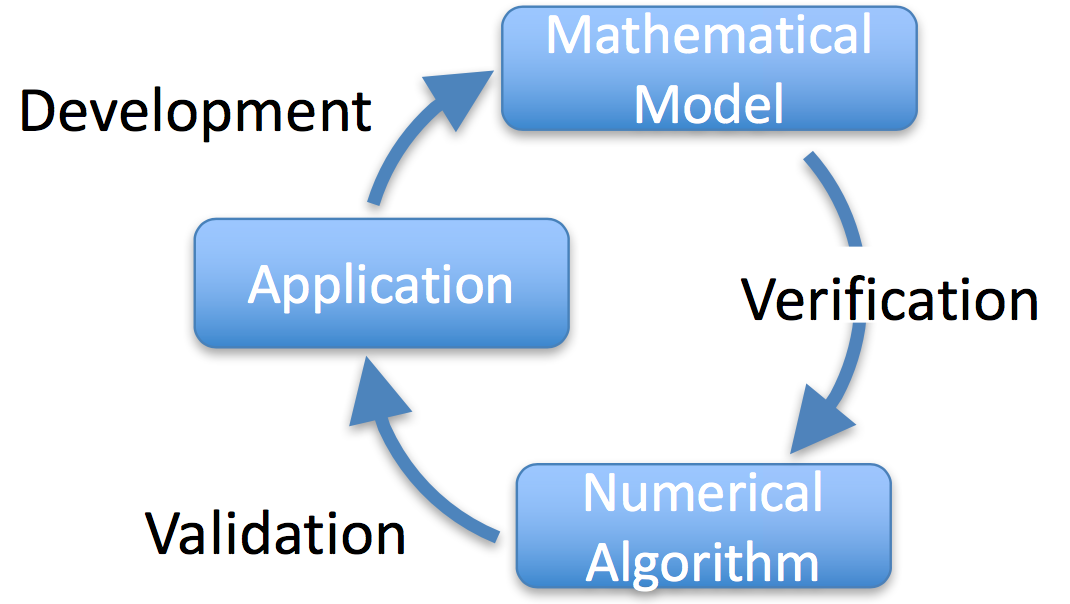
\includegraphics[height=2in]{Figures/vv_cycle.png}
\caption{Schematic representation of the verification and validation process used to evaluate the accuracy of a computational model. Adapted from \cite{Oberkampf:2010}.}
\label{fig:vv_cycle}
\end{figure}

The prevailing technique for verification consists in comparing results of the computational model with analytical solutions (or manufactured solutions \cite{Oberkampf:2010}) obtained for the same system of governing equations. This is usually accomplished through the construction of a library of \emph{unit test} problems. These problems are selected to exercise certain parts of the code (for instance the flow solver --- with or without convection, with or without diffusion, --- the combustion solver, the radiation solver, {\it etc}), considered sequentially and in isolation. The library is constructed with the objective to attain as much ``code coverage'' with unit test problems as possible. Note that MaCFP is not concerned with verification and assumes that the CFD solvers selected for MaCFP activities have been and are continuously verified. MaCFP is focused on validation.

The prevailing technique for validation consists in comparing experimental data with results of the computational model obtained in the same configuration. The target experiments considered in MaCFP correspond to ``open" validation tests in which the modelers have unlimited access to the details of the setup and to the experimental data prior to running the model. In most simulations presented below, the CFD solvers are used in their baseline configuration (presented briefly in section~\ref{sec:PM}), $i.e.$, without resorting to any model modification or calibration, and the simulations can be therefore interpreted as true \emph{validation} tests. In the case of the UMD turbulent line flame experiments, the CFD solvers were used with some advanced features to describe flame extinction that may or may not be part of the baseline configurations. In addition, some of these advanced features were originally tuned against data obtained from the same UMD experiments. In that case, the simulations should be interpreted as \emph{calibration} tests rather than validation tests.

In this first edition of the MaCFP workshop series, no effort was made to impose particular metrics in the comparison between experimental data and simulation results. Comparisons generally take the form of plotting measured and simulated spatial profiles of mean or root-mean-square ({\it rms}) quantities (mean quantities refer to time-averaged quantities and {\it rms} quantities designate the square root of the mean squared deviation of a quantity from its mean). Also no effort was made to require systematic estimates of experimental or numerical uncertainties.

\subsubsection{Computational Grid Design}
\label{sec:CGD}

One of the main challenges found in the application of CFD tools to the simulation of complex flow problems is the design of the computational grid. In large eddy simulations (LES), the design of the computational grid comes from an analysis of the characteristic length scales of the problem and a requirement that large-scale features that (presumably) control the flow dynamics be captured by the grid. The implicit assumption is that small-scale features are dynamically controlled by the resolved scales and can be represented through subgrid-scale (SGS) models. Relevant large-scale features that are considered dynamically-controlling and are therefore grid-resolved in LES of turbulent diffusion flames include: the large flow structures responsible for the production of turbulent kinetic energy (their size is estimated by the integral length scale of the turbulent flow); the large wrinkles on the flame surface responsible for enhanced fuel-air mixing and heat release; and the large soot-containing structures inside and outside the flame zone responsible for flame emission and smoke absorption properties. Small-scale features that are considered dynamically-controlled and remain therefore grid-unresolved in LES include: the small flow structures responsible for the dissipation of turbulent kinetic energy (their size is estimated by the Kolmogorov length scale); the thin reactive layers that make up the micro-structure of a turbulent flame; and the thin elongated soot layers that make up the micro-structure of the flame radiation field.

While the discussion above provides a valuable framework, it is important to emphasize that the separation between large scales that are dynamically-controlling and small scales that are dynamically-controlled is somewhat artificial and is not necessarily obvious. For instance, let us consider the case of a simple pool flame fueled by a liquid chemical supplied through a circular burner of diameter $D$. The pool fire literature suggests that $D$ is the only relevant length scale of the problem: the mean flame vertical height, the mean flame horizontal thickness and the characteristic size of the large turbulent flow structures expected in the flame region are all proportional to $D$ and can be captured in a LES simulation provided that the grid spacing is 10-20 times smaller than $D$.

\begin{figure}
\centering
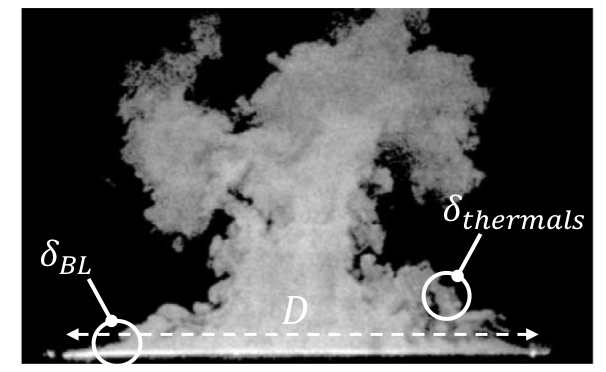
\includegraphics[height=2in]{Figures/He-Plume-Scales.png}
\caption{Illustration of the multi-scale nature of pool fire configurations using a flow visualization of the Sandia helium plume experiment. The configuration features: large-scale structures in the center of the plume with size on the order of the plume diameter $D$; thin boundary layers near the edges of the plume with size $\delta_{BL}$; and small structures created by Rayleigh-Taylor instabilities with size $\delta_{thermals}$. Adapted from \cite{Case1_EXP}.}
\label{fig:He-Plume-Scales}
\end{figure}

However, this is not the whole story. In many cases, the pool flame features a strong buoyancy-driven instability (called the puffing instability) that results in large oscillations in the (horizontal) entrained air flow and the (vertical) combustion products flow. Under strongly unstable conditions, the instantaneous flame takes different shapes during the instability cycle, including the shape of a somewhat unexpected thin (horizontal) boundary layer flame established close to the pool surface and produced by large peak values of the air flow velocity. The presence of the intermittent boundary layer flame is generally over-looked in pool fire studies but circumstantial evidence suggests that it plays an important dynamical role in the instability cycle and consequently needs to be correctly captured by the computational grid. Because its thickness $\delta_{BL}$ is much smaller than the pool diameter $D$, the simulation of the intermittent boundary layer flame brings stringent constraints to the design of the computational grid.

A related topic is the possible development of Rayleigh-Taylor instabilities in regions of the flame with unstable thermal stratification and the associated formation of small plume-like structures, often called ``thermals". When present, these thermals are believed to be responsible for enhanced fuel-air mixing and heat release. Because their characteristic size $\delta_{thermals}$ is much smaller than the pool diameter $D$, the simulation of the thermals brings additional stringent constraints to the design of the computational grid.

Figure~\ref{fig:He-Plume-Scales} presents an illustration of the multi-scale nature of pool fire configurations (albeit in the case of a chemically inert plume) and identifies the three dynamically-controlling length scales: $D$, $\delta_{BL}$ and $\delta_{thermals}$. The dynamic effects occurring at these length scales can be captured in a LES simulation provided that the grid spacing is 10 times smaller than $D$, $\delta_{BL}$ and $\delta_{thermals}$.

We now consider the implications of the previous discussion to the choice of grid resolution in LES simulations of the target experiments selected for the first MaCFP workshop. In the list of six target experiments (Cases 1-5 in section~\ref{sec:intro}), three correspond to pool-like configurations with significant buoyancy-driven instability phenomena ($i.e.$ strong puffing motions and the formation of thermals): the Sandia helium plume; the Sandia methane and hydrogen pool fires; and the UW methanol pool fire. The flow visualization techniques used in these experiments reveal intermittent boundary layers and thermals with length scales on the order of 1~cm, which based on the discussion above, suggests that a millimeter-scale computational grid may be required for accurate simulations. In addition, one target experiment corresponds to a boundary layer flame configuration: the FM Global vertical wall flame. The flow visualization techniques used in this experiment reveal boundary layers and structures with length scales on the order of 1~cm, which again suggests using a millimeter-scale computational grid. Finally, two target experiments correspond to pool-like configurations without reported evidence of a controlling puffing instability: the NIST McCaffrey natural gas flames and the UMD methane and propane turbulent line flames. In the case of the NIST McCaffrey experiments, the only apparent characteristic length scale is the burner size (0.3~m), which suggests using a centimeter-scale computational grid. In the case of the UMD experiments, the only apparent characteristic length scale is the burner width (5~cm), which suggests using a millimeter-scale computational grid.

Note that the numerical submissions to the first MaCFP workshop generally correspond to grid resolutions consistent with the estimates above. In this first edition of the MaCFP workshop series, no effort was made to require systematic grid convergence studies.

\subsubsection{Physical Modeling}
\label{sec:PM}

The numerical submissions to the first MaCFP workshop correspond to one of the following four CFD solvers: FDS, FireFOAM, ISIS and SIERRA/Fuego. All four models are used in LES mode. The solvers differ in details of the formulation of the governing equations, in the construction of the computational grid, in the choice of algorithms used to discretize the governing equations and to provide a numerical solution, and in their ability to perform parallel computing. These differences are believed to be inconsequential in the present tests because the simulations correspond to simple academic configurations. The solvers also differ in the formulation of the physical models used to describe subgrid-scale turbulence, combustion and radiation. These differences are believed to be significant and may be responsible for some or many of the reported discrepancies observed between simulation results, as summarized in the following sections.

In their baseline configuration, the four CFD solvers use:
\begin{itemize}
\item For subgrid-scale turbulence: a classical gradient transport formulation with a SGS turbulent viscosity. A closure expression for the SGS turbulent viscosity is provided by: a modified Deardorff model~\cite{Deardorff:1980} (FDS, see also Ref.~\cite{FDS_Math_Guide}); a model using a (constant-coefficient or dynamic) equation for SGS turbulent kinetic energy~\cite{Fureby:1997} (FireFOAM, SIERRA/Fuego); or the dynamic Smagorinsky model~\cite{Moin:1991} (ISIS).
\item For combustion: a global combustion equation combined with a closure expression for the reaction rates based on either the Eddy Dissipation Model~\cite{Magnussen:1976} (FDS, see also Ref.~\cite{FDS_Math_Guide}, FireFOAM, ISIS) or a steady laminar flamelet model~\cite{SIERRA/Fuego_User_Guide1,SIERRA/Fuego_User_Guide2} (SIERRA/Fuego).
\item For radiation: a treatment based on either a solution of the radiative transfer equation (RTE) combined with a closure expression for the emission term using a prescribed global radiative loss fraction (FDS, see also Ref.~\cite{FDS_Math_Guide}, FireFOAM) or a solution of simplified equations based on the $P$1-approximation (ISIS)  (note that results obtained with SIERRA/Fuego did not use a radiation model).
\end{itemize}

These baseline models have a number of known limitations. First, the SGS turbulence models are models that have been formulated for high-Reynolds-number, momentum-driven flow applications and that may not apply directly to fires which feature moderate-Reynolds-number, buoyancy-driven flow and Rayleigh-Taylor instabilities. Second, the combustion models based on a global combustion equation and the Eddy Dissipation Model are limited to configurations without ignition/extinction phenomena and need to be modified to treat flame extinction in applications to under-ventilated fires or suppressed fires. And third, the radiation models based on a prescribed global radiative loss fraction are limited to configurations in which these fractions have been measured and in which the fire regime does not deviate significantly from the conditions of the measurements.

The identification of these limitations, the quantification of their relative importance, and ultimately their elimination through more advanced models are some of the objectives of the MaCFP effort.























% !TEX root = macfp_2017_gasphase.tex

\subsection{Case 1: Turbulent Buoyant Plumes} \label{sec:buoyant_plumes}

\subsubsection{Experiment}

The buoyant plume experiment selected for the first MaCFP workshop is a turbulent non-reacting helium plume studied at a test facility called the Fire Laboratory for the Accreditation of Models by Experimentation (FLAME) facility at Sandia National Laboratories~(Sandia)~\cite{Blanchat:2001,Case1_EXP}. The original goal of the Sandia buoyant plume experiment was to provide comprehensive turbulent flow velocity and species concentration statistics in a configuration that is representative of large-scale pool fires without the complexities of chemical reactions and temperature variations~\cite{Case1_EXP}.  The 1-m diameter source provides a plume in the fully-developed turbulent flow regime.  

The 1-m diameter helium source was surrounded by a 0.51-m wide steel lip, representing the injection plane and elevated 2.45 m above an annular ring which introduced a low-velocity co-flow of ambient air~\cite{Blanchat:2001}. The FLAME facility can be approximated as a 6.1-m cubic chamber covered by a 2.4-m diameter extraction hood. Planar imaging measurements of velocity and species were conducted using Particle Image Velocimetry and Planar Laser Induced Fluorescence, respectively. Laser measurements were recorded at 200~Hz in a window approximately 0.86~m high and 1.2~m wide, and providing an image of the near-field region (starting from the helium injection plane and centered on the plume centerline). The measurement window includes near-field entertainment zones on both sides of the plume; however, it does not include the lateral and vertical far-field. The experimental uncertainty of the measured velocities and turbulent statistics are reported as 20\% and 30\%, respectively. The uncertainty of the measured helium concentration is reported as 18\%. Inlet conditions are uniform to within 5\% or less for the helium flow and within 10\% for the air coflow. The above uncertainties include run-to-run variability. 

For the purpose of MaCFP, tests no. 25, 29, 32 and 36 were selected corresponding to repeat runs with a helium inlet velocity of 0.339 m/s $\pm 1.3$\%, a flow Reynolds number $Re=3194$~$\pm$ $0.6$\%, a flow Richardson number $Ri=69.53$~$\pm 6.5\%$ and a measured puffing frequency of $1.45$ Hz \cite{Case1_EXP}.

\subsubsection{Simulations}

Three groups submitted computational results for Case 1:  IRSN~\cite{Case1_SIM_IRSN}, NIST~\cite{Case1_SIM_NIST} and UGent~\cite{Case1_SIM_UGent}. Some information was also compared with past results published in the literature by Sandia running Fuego~\cite{DesJardin:2004}. IRSN used ISIS version 4.8.0~\cite{ISIS}; NIST used an official release of FDS (version 6.5.3)~\cite{FDS}; UGent used FireFOAM version 1.6~\cite{FireFOAM}.

As discussed in section~\ref{sec:CGD}, the main challenge found in the design of a computational grid for LES simulations of the Sandia helium plume experiment is to provide suitable grid resolution to capture the intermittent boundary layer and ``thermals" that result from unstable buoyant motions (see Figure~\ref{fig:He-Plume-Scales}). This may require millimeter-scale resolution. The computational groups responded to this challenge in different ways: IRSN adopted a 2.5-cm resolution; NIST adopted a 1.5-cm resolution; UGent adopted a stretched grid with 1.23-cm resolution near the helium source. Note that previous work in Ref.~\cite{DesJardin:2004} used both 3- and 5-cm grid resolution. The computational domain in all simulations is much larger than the measurement region (and is 3- or 4-m wide and 4-m high); however, it does not include all details of the full facility. 

Note that there were some variations among computational groups in the treatment of the co-flow: the air co-flow velocity was introduced through an annular ring located below the helium injection plane with a ring-level velocity approximately equal to 0.15-0.18~m/s~\cite{Blanchat:2001}; IRSN did attempt to model the annular ring but did not use the correct geometry and coflow velocity; in contrast, NIST and UGent did not attempt to model the annular ring and assumed instead simplified boundary conditions at the helium injection plane \-- NIST prescribed a small coflow velocity equal to 0.01~m/s (at the injection plane) while UGent used free entrainment conditions. Also, while NIST and UGent assumed an ambient pressure of 80.9~kPa (due to the high elevation of the FLAME facility), IRSN incorrectly assumed an ambient pressure of 101.1 kPa.

\begin{figure}
\centering
(a)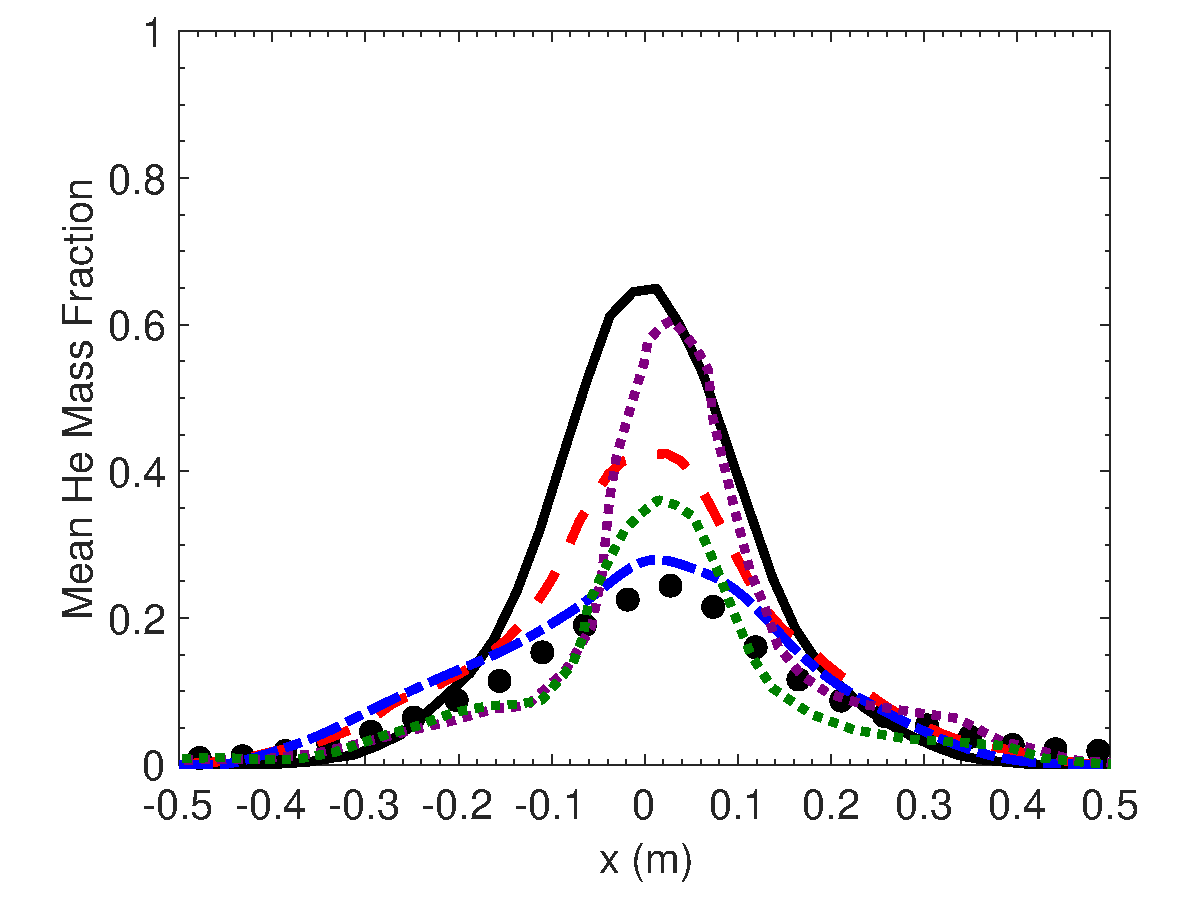
\includegraphics[height=2.2in]{Figures/Case1-Fig1a.pdf}
(b)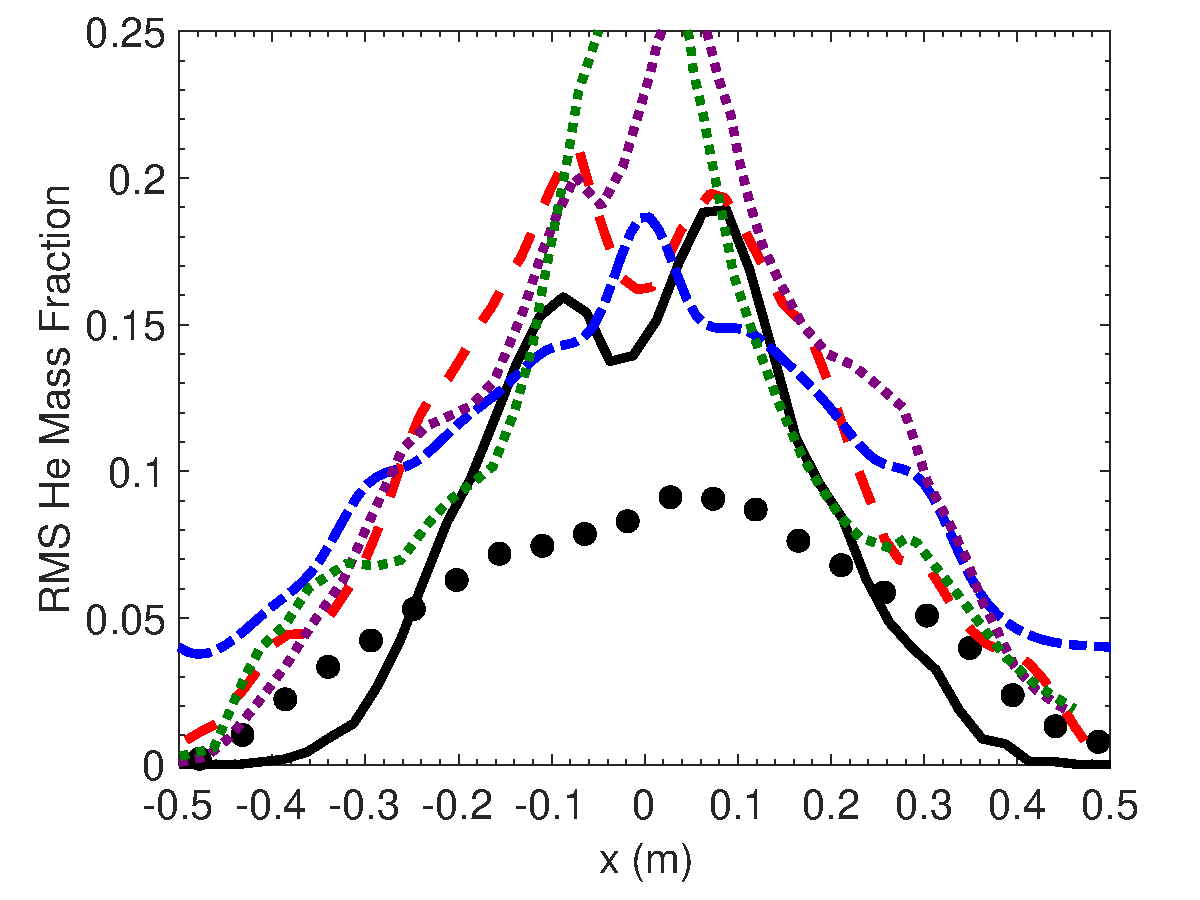
\includegraphics[height=2.2in]{Figures/Case1-Fig1b.pdf}
(c)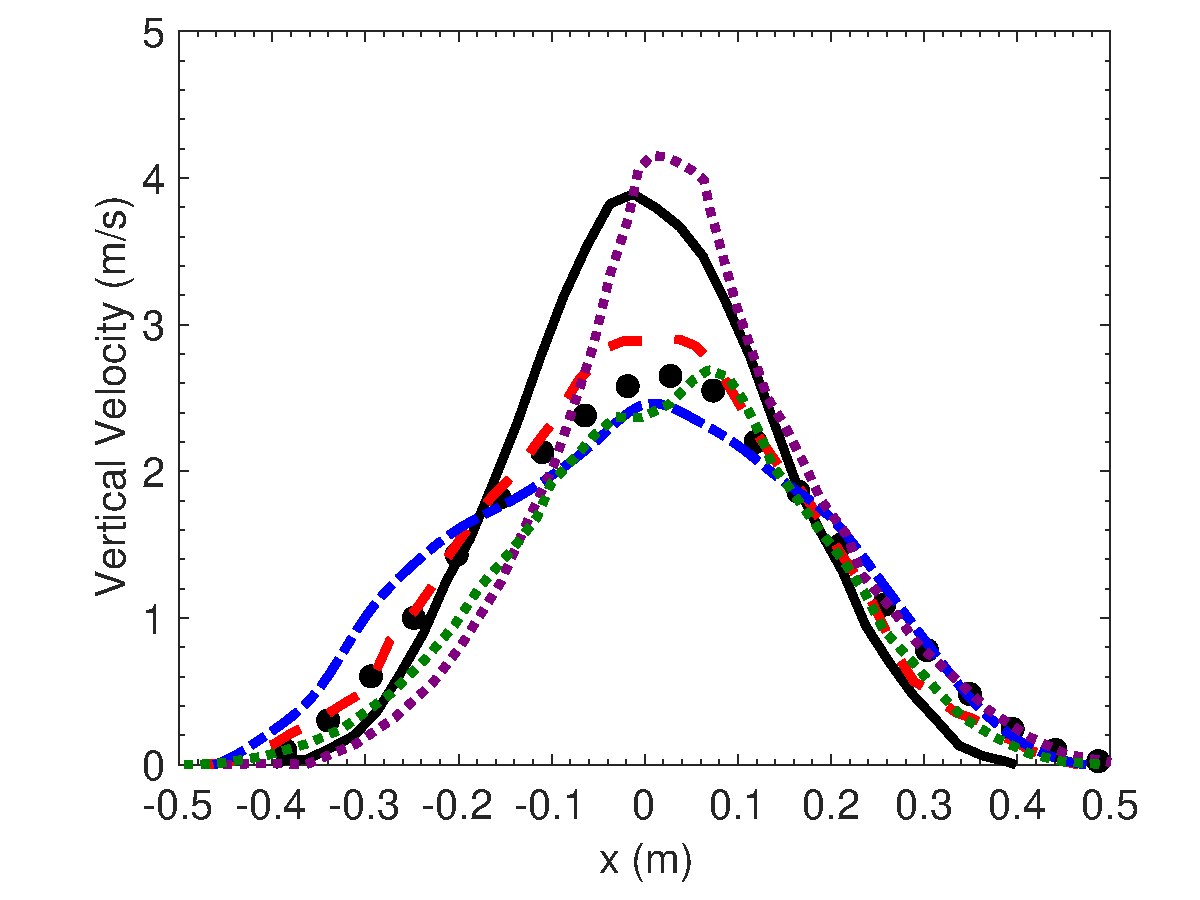
\includegraphics[height=2.2in]{Figures/Case1-Fig1c.pdf}
(d)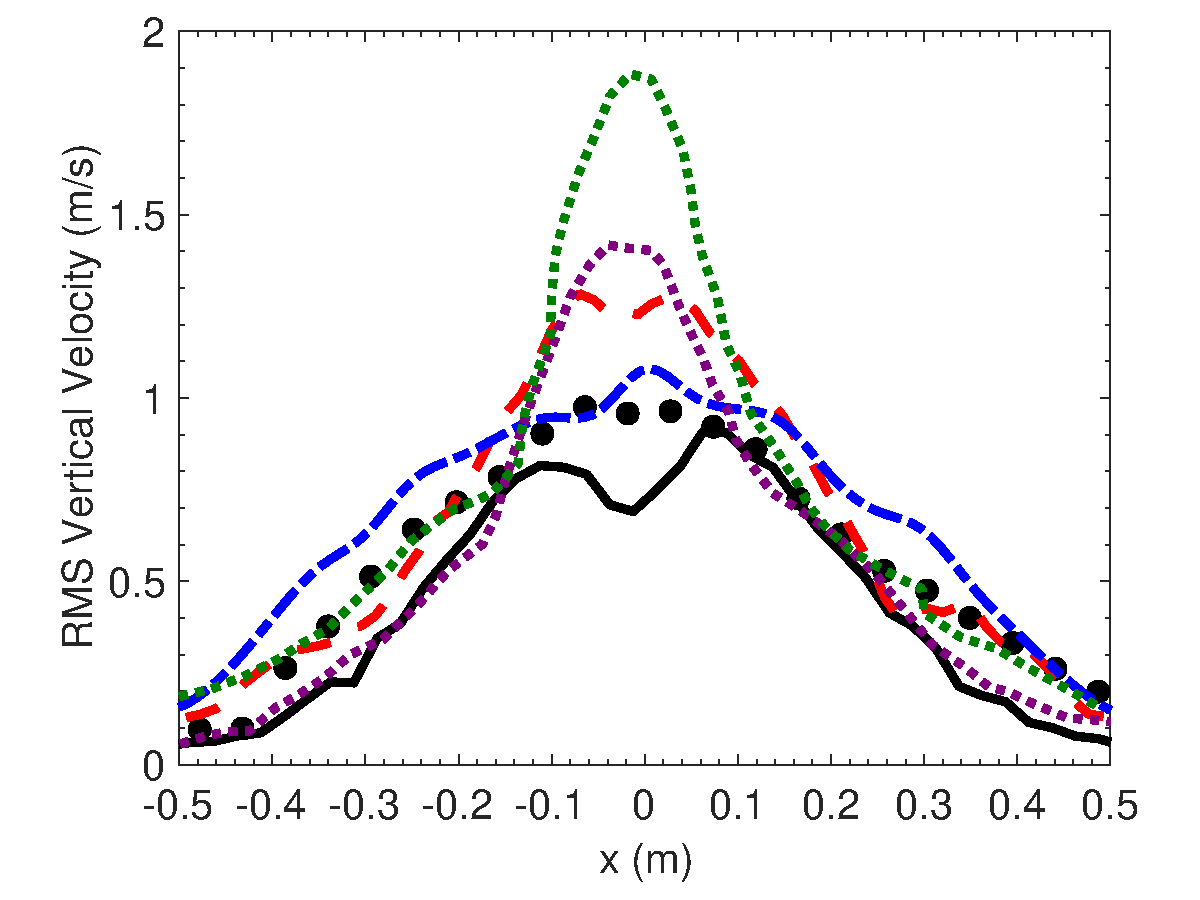
\includegraphics[height=2.2in]{Figures/Case1-Fig1d.pdf}
\caption{Case 1. Radial variations at $z = 0.4$~m of: (a) mean helium mass fraction; (b) {\it rms} helium mass fraction; (c) mean vertical velocity; (d) {\it rms} vertical velocity. Comparison between experimental data (black circles) and numerical results from IRSN (black solid line), NIST (red dashed line), UGent (blue dash-dotted line) and results from Ref.~\cite{DesJardin:2004} (magenta and green dotted lines, corresponding to 5-cm and 3-cm resolution, respectively).}
\label{fig:Case1-Fig1}
\end{figure}

Additional differences in the numerical treatment of the Sandia plume experiment include differences in the choice of physical models (see section~\ref{sec:PM} for details on baseline choices).  IRSN used the baseline configuration of ISIS and NIST used the baseline configuration of FDS. UGent deviated from baseline choices in FireFOAM and used the constant-coefficient Smagorinsky model for subgrid-scale turbulence (additional information can be found in Ref.~\cite{Maragkos:2013}). 

The durations of the simulations and the durations over which numerical results were collected and statistical moments were evaluated varied: IRSN, NIST and UGent chose to run their models for 10~s, 20~s and 30~s, respectively (in Ref.~\cite{DesJardin:2004}, the model was run for 20~s); all groups except IRSN chose to collect numerical results over the last 10~s, corresponding to approximately 14 puffing cycles; IRSN analyzed data over 3~s or approximately 4 puffing cycles (in this case, the results should be analyzed with caution because the statistics may not be converged) .

\subsubsection{Summary}

Figure~\ref{fig:Case1-Fig1} presents a representative sample of comparisons between measured and simulated helium mass fractions and vertical flow velocity. The comparisons generally suggest that accuracy increases with higher levels of grid resolution and that an accurate description of the flow statistics in the near-field region requires a resolution of approximately 1 or 2~cm. Note that this corresponds to 100 or 50 computational cells across the source diameter, a level of resolution that is much higher than the usual requirement of providing a grid spacing that is 10-20 times smaller than the source diameter $D$. In addition, even at this high level of resolution, the magnitude of the fluctuations in helium mass fraction is not captured accurately (see Figure~\ref{fig:Case1-Fig1}(b)). These inconsistent results suggest that the dynamics associated with the presence of both thin boundary layers near the edges of the helium source and small-scale ``thermals" generated by secondary buoyant instabilities play a significant role in determining near-field turbulent mixing properties. Note that the exact impact of the inaccuracies in the near-field on the global flow features of the far-field have not been characterized.

It is worth emphasizing that the experimental database describing the Sandia helium plume experiment is of great value because it contains data on first and second-order statistical moments of flow velocities and helium concentrations measured with high spatial resolution~\cite{Case1_EXP}. There are also some limitations in the database that are worth pointing out for future studies: (1) the Sandia database is limited to the plume near-field, $i.e.$ to low elevations ($z \leq 1.2$~m, $i.e.$ $z < (1.2 \times D$)), and there is a need to provide similar data in the far-field; (2) the Sandia database does not provide much information on the puffing cycle and there is a need to provide phase-averaged data to characterize the coupling between large- and small-scale dynamics.



% !TEX root = macfp_2017_gasphase.tex

\subsection{Case 2: Turbulent Pool Fires with Gaseous Fuel} \label{sec:gaseous_pool_fires}

\subsubsection{Experiments}

The gaseous pool fire experiments selected for the first MaCFP workshop correspond to a series of natural gas flame experiments (Case 2a) studied at the National Institute of Standards and Technology (NIST)~\cite{Case2a_EXP} and a series of methane and hydrogen pool fire experiments (Case 2b) studied at Sandia National Laboratories (Sandia)~\cite{Case2b_EXP_CH4,Case2b_EXP_H2}. The original goal of the NIST McCaffrey natural gas flame experiment was to provide data to establish and/or validate engineering correlations for mean temperature and mean vertical flow velocity along the center line of pool fires. The original goal of the Sandia methane and hydrogen pool fire experiment was to provide comprehensive turbulent flow velocity statistics in a configuration that is representative of large-scale pool fires.

The McCaffrey burner is a small-scale (0.3~$\times$~0.3)~m$^2$ square burner; in Ref.~\cite{Case2a_EXP}, the total heat release rate was varied between 14.4 and 57.5~kW. Measurements of temperature and vertical flow velocity were made using thermocouples and bi-directional probes. The Sandia burner is a 1-m-diameter round burner located in a facility that can be approximated as a 6.1~m cube covered by an extraction hood; in Refs.~\cite{Case2b_EXP_CH4,Case2b_EXP_H2}, the total heat release rate was MW-scale (for the purpose of MaCFP, tests no. 14, 24, 17 and 35 were selected corresponding to methane flames with a total heat release rate equal to 1.59, 2.07 and 2.61~MW, and to a hydrogen flame with a total heat release rate equal to 2.12~MW, respectively). The Sandia flames featured strong puffing motions and the formation of thermals. Flow velocities were measured using Particle Image Velocitimetry; starting from the burner surface, measurements were made at high resolution (with a spacing of 2~cm) and over a region approximately 0.9 m~high and 1~m wide. Estimates of errors in mean velocities for tests no. 14, 24, 17 and 35 range between 13\% and 23\%; estimates of errors in {\it rms} velocities range between 13\% and 28\%.

\subsubsection{Simulations}

Four groups submitted computational results for Case 2a: FM Global~\cite{Case2a_SIM_FMG}, UGent~\cite{Case2a_SIM_UGent}, IRSN~\cite{Case2a_SIM_IRSN} and NIST~\cite{Case2a_SIM_NIST}. Four groups submitted computational results for Case 2b: UGent~\cite{Case2b_SIM_UGent}, NIST~\cite{Case2b_SIM_NIST}, SNL~\cite{Case2b_SIM_SNL} and the UCantabria~\cite{Case2b_SIM_UCantabria}. FM Global used a shared development version of FireFOAM (FireFOAM-dev)~\cite{FireFOAM}; UGent used FireFOAM version 2.4.x (Case 2a) and version  2.2.x (Case 2b)~\cite{FireFOAM}; IRSN used ISIS version 4.8.0~\cite{ISIS}; NIST and UCantabria used an official release of FDS (version 6.5.3)~\cite{FDS}; SNL used SIERRA/Fuego version 4.44~\cite{SIERRA/Fuego}.

As discussed in section~\ref{sec:CGD}, the main challenge found in the design of a computational grid for LES simulations of the NIST McCaffrey flame experiment is to provide suitable grid resolution to capture the flow and flame features with length scales comparable to the burner size. All groups responded to this challenge in similar ways: FM Global and UGent adopted a 1.25-cm resolution in the flame zone; IRSN adopted a 1-cm resolution; NIST adopted a 1.43-cm resolution. Furthermore, as discussed in section~\ref{sec:CGD}, the dynamics of the Sandia pool fire experiment are apparently more complex and the main challenge found in the design of a computational grid for LES simulations is to provide suitable grid resolution to capture the intermittent boundary layer flame and thermals that result from the puffing instability. This may require millimeter-scale resolution. Given the high computational cost associated with simulations of meter-size configurations with millimeter-scale resolution, the computational groups responded to this challenge in different ways: UGent and NIST adopted a 1.5-cm resolution in the flame zone; SNL presented results obtained with a 2.5-cm and a 4-cm resolution; UCantabria adopted a 5-cm resolution. Note that while UGent and NIST decided to limit the computational domain to a subset of the experimental facility, SNL and UCantabria chose to include details of the full facility, including the co-flow arrangement and the extraction hood.

Additional differences in the numerical treatment of the NIST McCaffrey and Sandia pool fire experiments include differences in the choice of physical models (see section~\ref{sec:PM} for details on baseline choices). For Case 2a, FM Global used the baseline configuration of FireFOAM except for using a slightly simplified radiation treatment in which emission losses are correctly included in the energy equation (using the global radiative loss fraction concept) but radiation transport is ignored ($i.e.$ the RTE equation is not solved) because comparisons to experimental data do not require the evaluation of a heat flux at a remote surface; the values of the global radiative loss fraction were prescribed using the measured values (varying between 17\% and 27\%). UGent also used the baseline configuration of FireFOAM except for using the dynamic Smagorinsky model~\cite{Moin:1991} for subgrid-scale turbulence; the value of the global radiative loss fraction was prescribed as equal to 20\%; in the solution of the RTE, the discretization of angular space used 48 angles. IRSN used the baseline configuration of ISIS. NIST used the baseline configuration of FDS: the values of the global radiative loss fraction were prescribed using the measured values; in the solution of the RTE, the discretization of angular space used 104 angles.

For Case 2b, UGent used the baseline configuration of FireFOAM except for using the constant-coefficient Smagorinsky model for subgrid-scale turbulence and an emission/absorption treatment of the RTE for radiation combined with a grey model (for methane flames, the global radiative loss fraction was predicted to be equal to 24.8\%); in the solution of the RTE, the discretization of angular space used 48 angles (additional information can be found in Ref.~\cite{Maragkos:2017}). NIST and UCantabria used the baseline configuration of FDS (except that UCantabria used the Vreman model~\cite{FDS_Math_Guide} for subgrid-scale turbulence): the value of the global radiative loss fraction was prescribed as equal to 20\% (for methane flames) or 10\% (for hydrogen flames); in the solution of the RTE, the discretization of angular space used 104 angles. SNL used the baseline configuration of SIERRA/Fuego (but without radiation).

\begin{figure}
\centering
(a)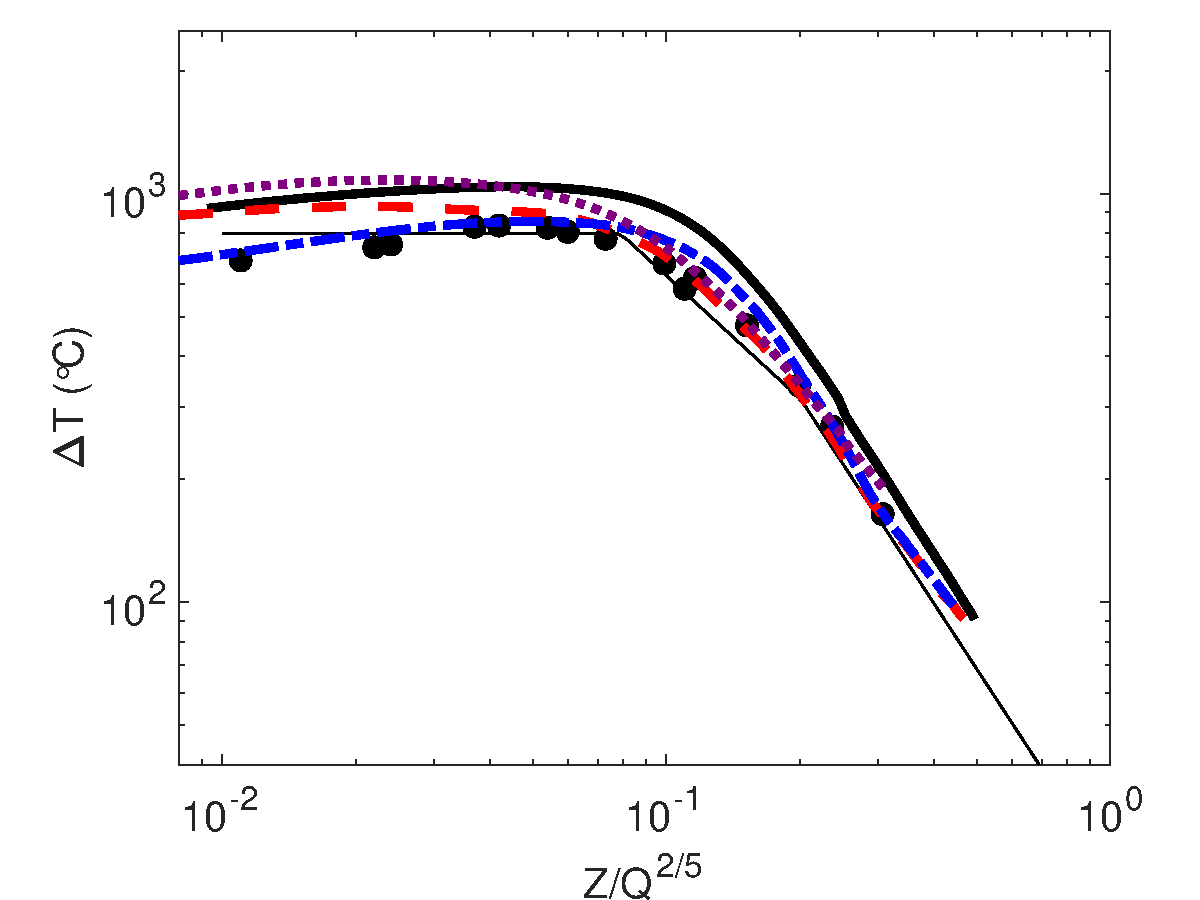
\includegraphics[height=2.2in]{Figures/Case2-Fig1a.pdf}
(b)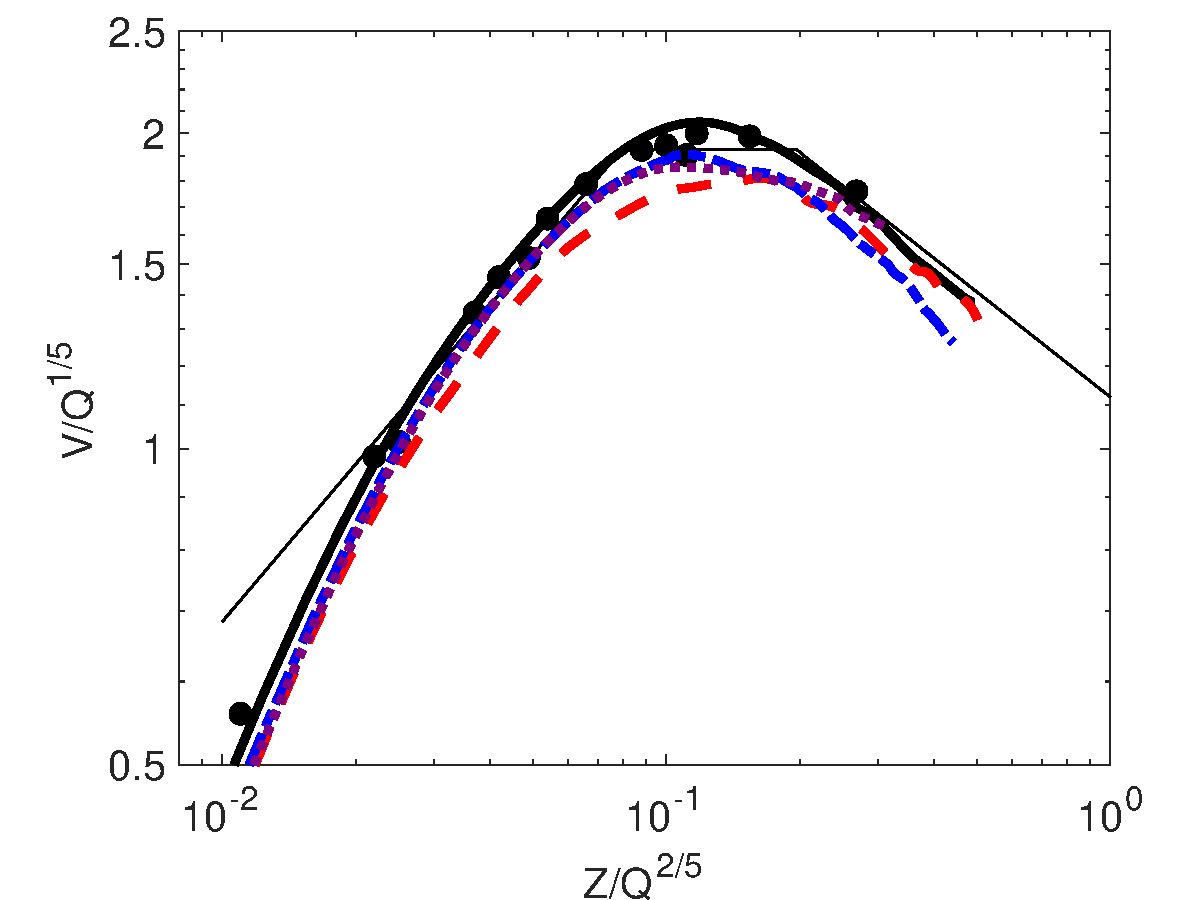
\includegraphics[height=2.2in]{Figures/Case2-Fig1b.pdf}
\caption{Case 2a. Vertical variations along the pool centerline (log-log plot): (a) mean excess temperature; (b) mean vertical velocity. Following standard scaling laws, vertical elevation is scaled by ${Q}^{2/5}$ while velocity is scaled by ${Q}^{1/5}$, with $Q$ the total heat release rate. Comparison between experimental data (black circles), engineering correlations (thin black solid line, see Ref.~\cite{Case2a_EXP}) and numerical results from FM Global (black solid line), IRSN (red dashed line), NIST (blue dash-dotted line), UGent (magenta dotted line). Case of a 33-kW flame.}
\label{fig:Case2-Fig1}
\end{figure}

\subsubsection{Summary}

For Case 2a, all simulations seem to correctly reproduce the gross features of the flame structure observed in the NIST McCaffrey flame experiment. Figure~\ref{fig:Case2-Fig1} presents a representative sample of comparisons between measured and simulated temperatures and vertical flow velocity. Note that in the NIST McCaffrey experiment, thermocouple measurements were not corrected for radiation losses and therefore should be interpreted with caution. NIST is the only computational group that used a thermocouple model to provide a sound basis for comparisons to the raw thermocouple measurements (the model is integrated inside the LES solver and uses the LES solution to simulate deviations of thermocouple temperatures from gas temperatures~\cite{FDS_Math_Guide}); other groups reported gas temperatures that require a correction before making a comparison to the raw thermocouple measurements.

It is worth emphasizing that while the experimental database describing the NIST McCaffrey natural gas flame experiment is a valuable starting point for model validation, there are, however, some obvious limitations in the database that are worth pointing out for future studies: (1) the database is limited to small-scale, weakly-to-moderately turbulent flames; and (2) the database is limited to temporal means and does not contain information on fluctuation magnitudes.

We now proceed to a discussion of Case 2b. All simulations seem to correctly reproduce the gross features of the flame structure observed in the Sandia pool fire experiment. Figures~\ref{fig:Case2-Fig2}-\ref{fig:Case2-Fig3} present a representative sample of comparisons between measured and simulated mean vertical and radial velocities. Mean radial velocities are particularly important because they provide a measure of the air entrainment process that determines the vertical mass flow rate in the flame and plume regions (and thereby controls smoke production in fires): for instance, Figure~\ref{fig:Case2-Fig3} shows that at the edge of the pool fire ($i.e.$ at 0.5-m distance from the center of the burner), the radial velocity is over-estimated by a factor close to two in the SNL and UCantabria simulations (at $z = 0.3$~m). Additional comparisons can be found in~\cite{MaCFP_wks_presentations}. Overall, the UGent and NIST simulations show good agreement with experimental data and provide a satisfactory description of the flame structure. The accuracy of the UCantabria simulation is limited by insufficient grid resolution. 

It is worth emphasizing that the experimental database describing the Sandia methane and hydrogen pool fire experiment is quite unique because it contains data on first and second-order statistical moments of vertical/radial velocities measured with high spatial resolution~\cite{Case2b_EXP_CH4,Case2b_EXP_H2}. There are also some limitations in the database that are worth pointing out for future studies: (1) the Sandia database is limited to the flame near-field, $i.e.$ to low elevations ($z \leq 0.9$~m, $i.e.$ $z < D$), and there is a need to provide data over the full flame region ($0 \leq z \leq L_f$); (2) the Sandia database focuses on the flow structure in the flame region but does not contain information on the temperature and radiation fields.

Finally, it is also worth noting that while research-level simulations may accept the computational cost associated with millimeter- or centimeter-scale resolution, engineering-level simulations will not accept that cost and will use coarser grids ($i.e.$ grids that resolve length-scales on the order of the pool diameter $D$, but not the smaller length scales associated with a boundary layer flame or the presence of thermals). These coarser-grid simulations require accurate subgrid-scale models: the evaluation of current SGS models in simulations with representative engineering-level grids was not part of the scope of the first MaCFP workshop and will be addressed in future editions.


\begin{figure}
\centering
(a)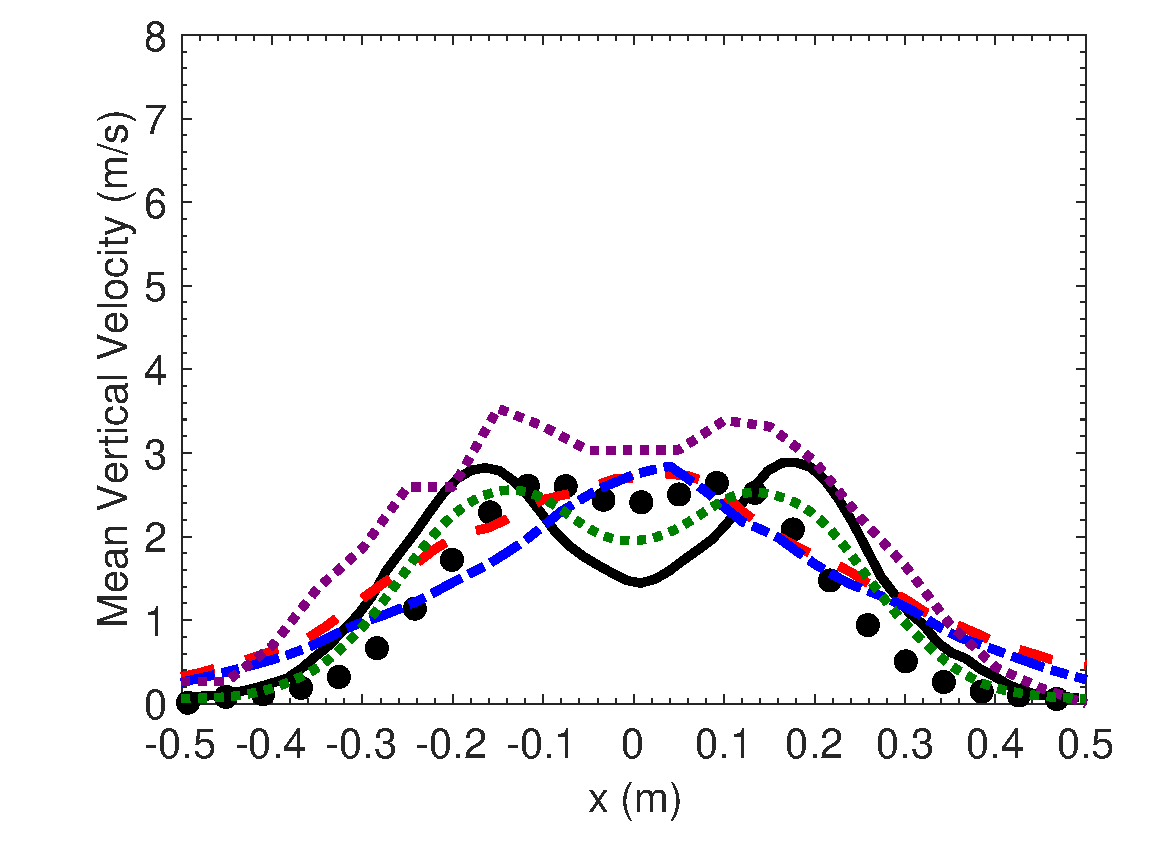
\includegraphics[height=2.2in]{Figures/Case2-Fig2a.pdf}
(b)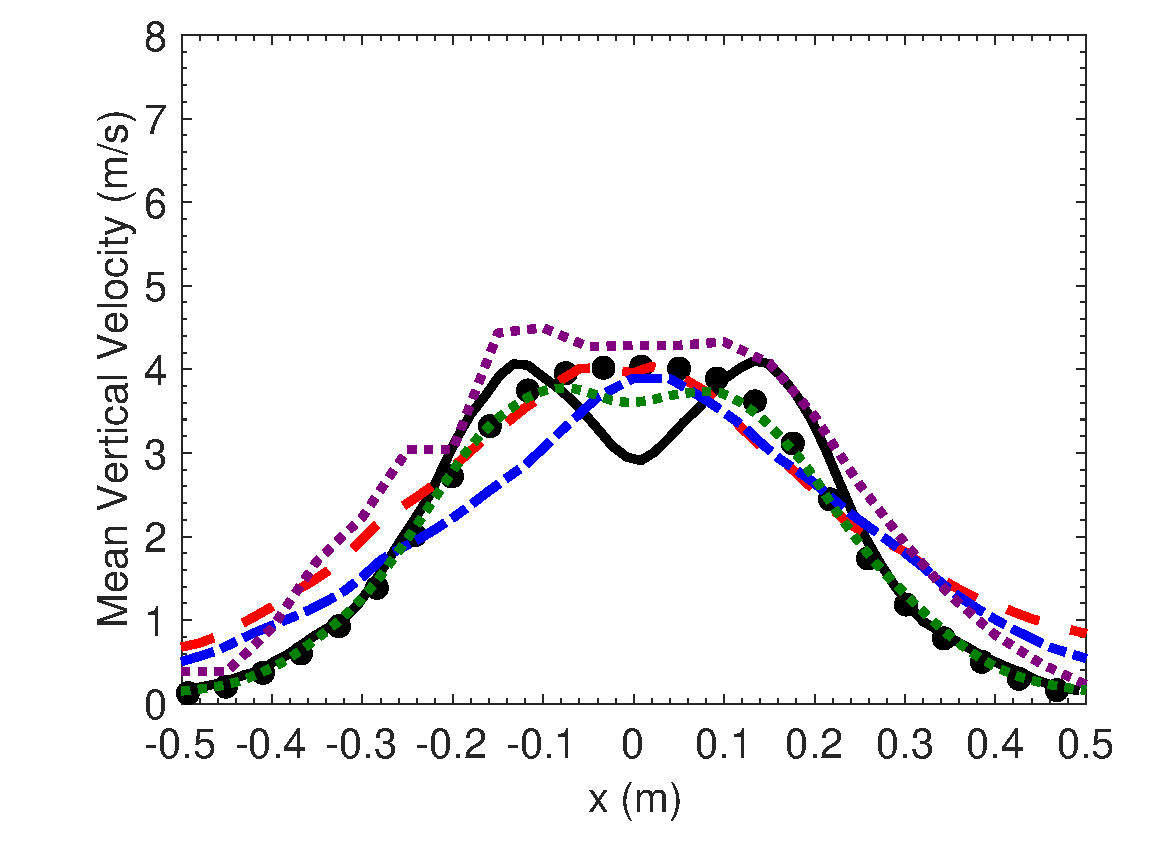
\includegraphics[height=2.2in]{Figures/Case2-Fig2b.pdf}
(c)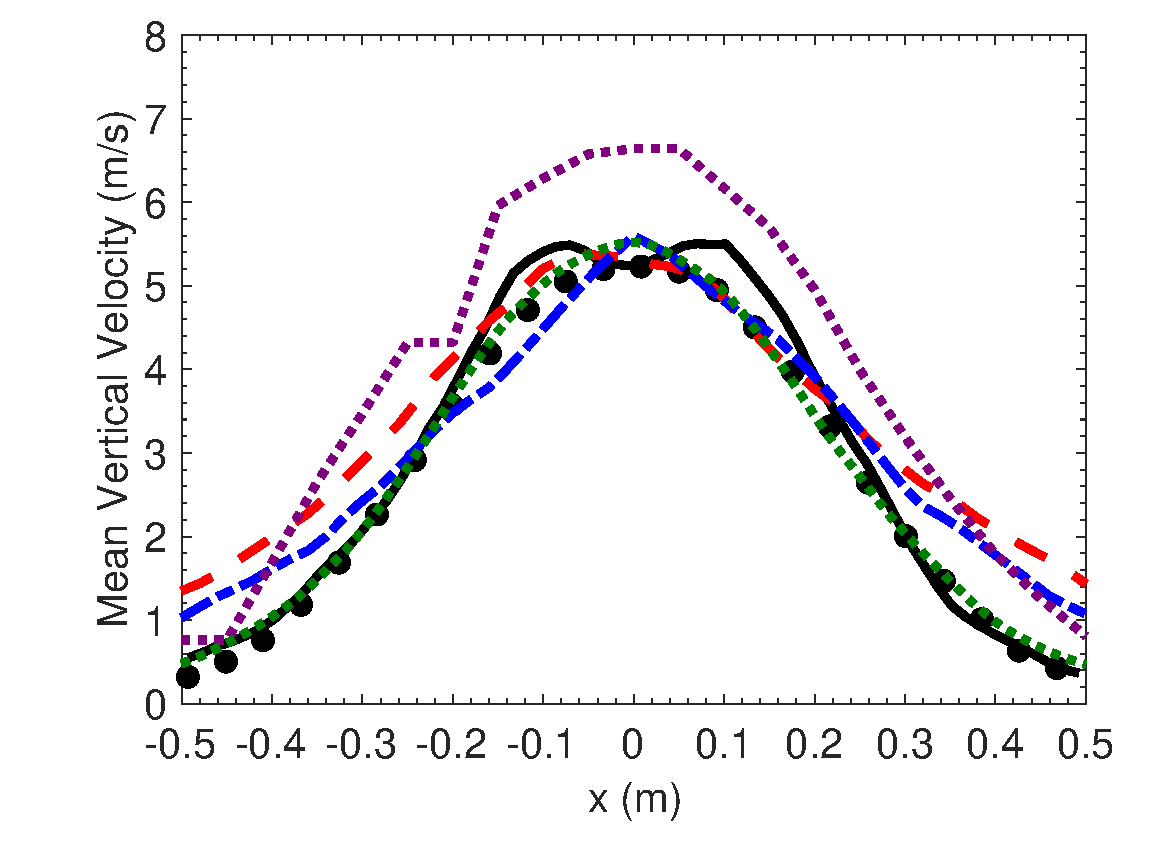
\includegraphics[height=2.2in]{Figures/Case2-Fig2c.pdf}
(d)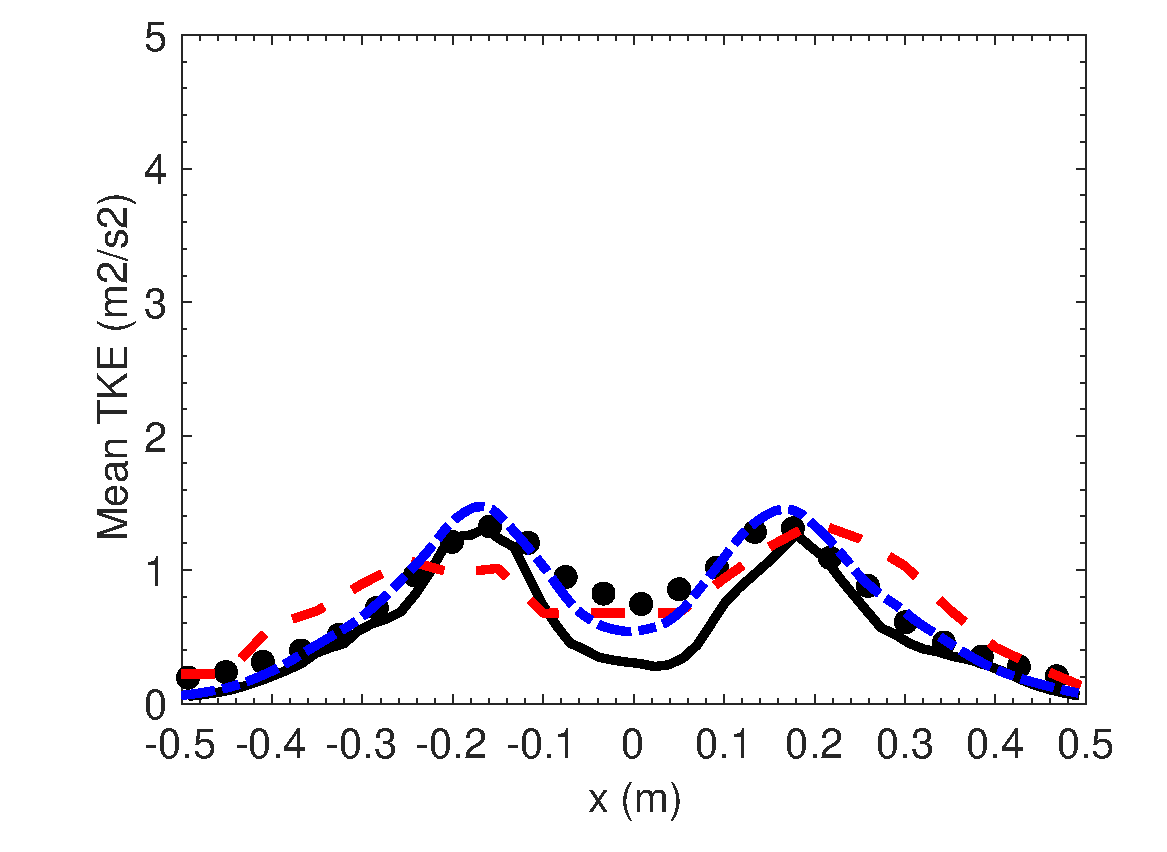
\includegraphics[height=2.2in]{Figures/Case2-Fig2d.pdf}
\caption{Case 2b. Radial variations of mean vertical velocity at elevation: (a) $z = 0.3~m$; (b) $z = 0.5~m$; (c) $z = 0.9~m$; and radial variations of mean (resolved) turbulent kinetic energy at $z = 0.5~m$. Comparison between experimental data (black circles) and numerical results from NIST (black solid line),  SNL (red dashed and blue dash-dotted  lines); UCantabria (magenta dotted line); UGent (green dotted line). Case of a 2.07-MW methane flame (test 24).}

\label{fig:Case2-Fig2}
\end{figure}
\begin{figure}
\centering
(a)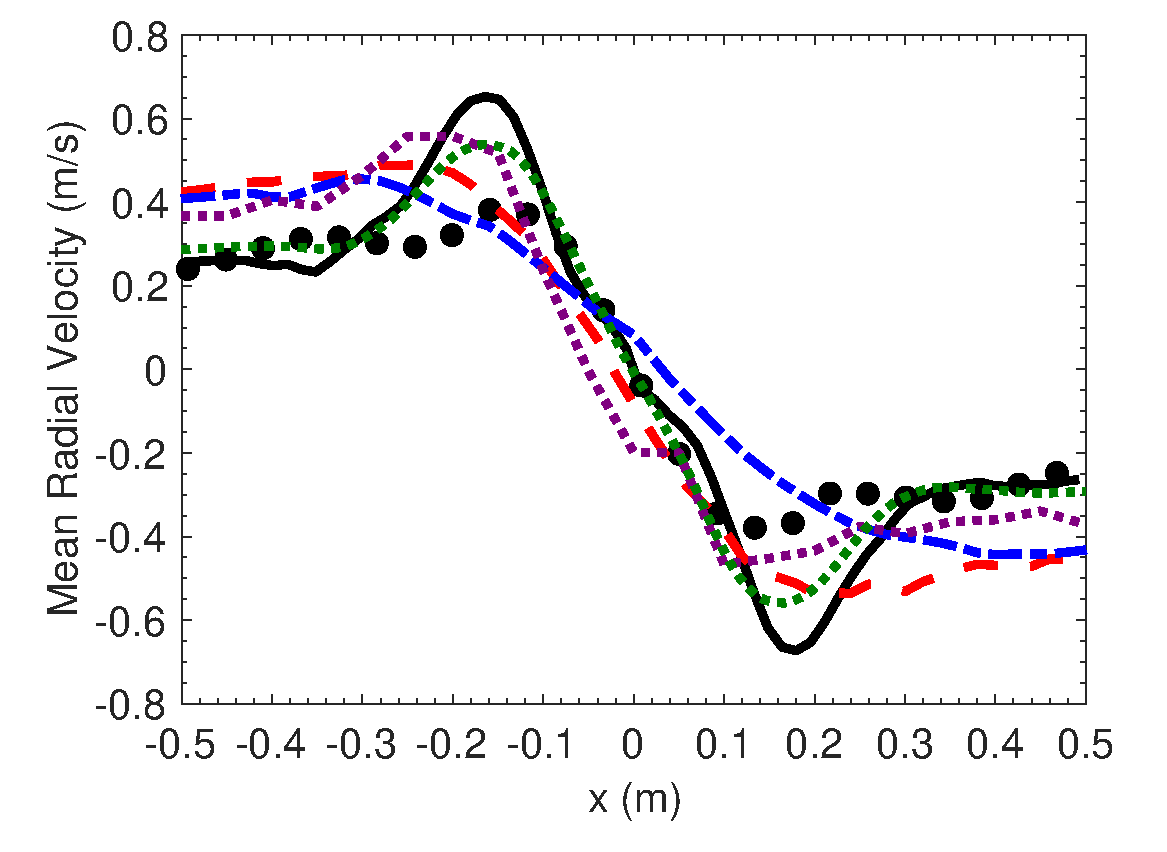
\includegraphics[height=2.2in]{Figures/Case2-Fig3a.pdf}
(b)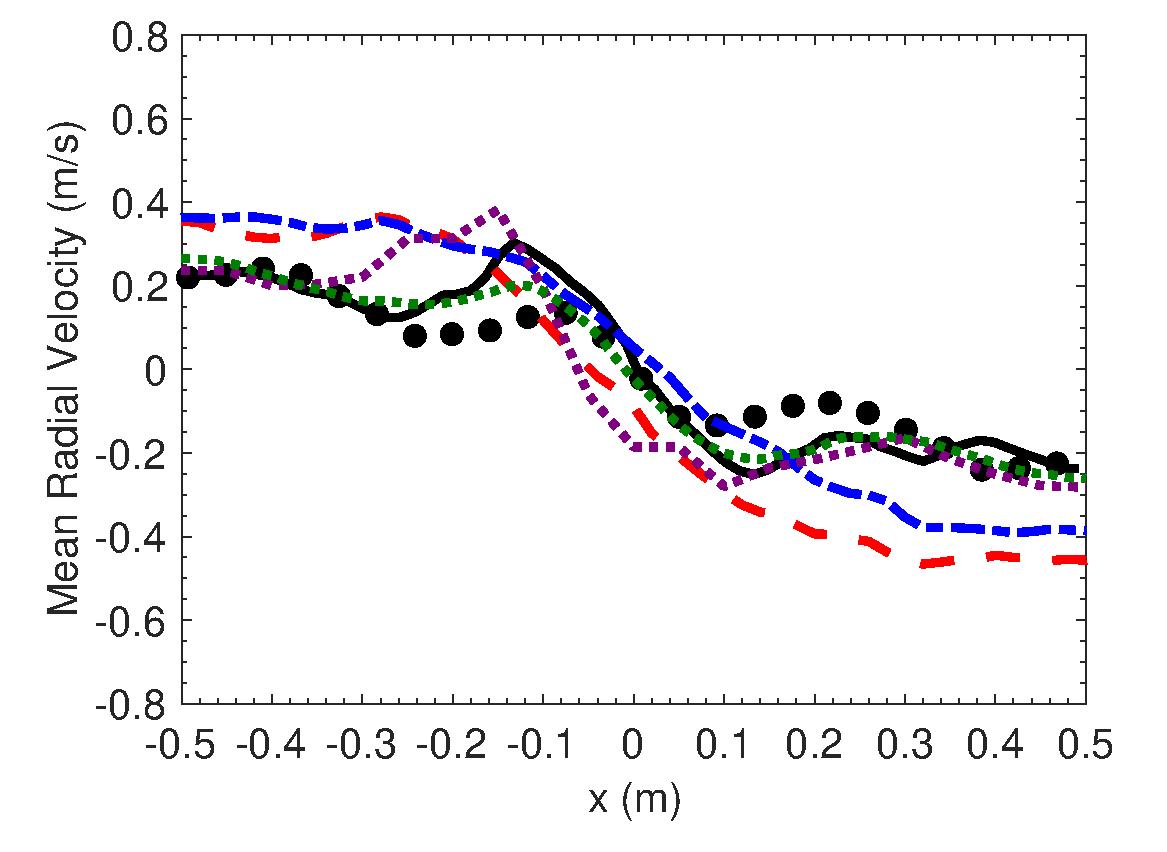
\includegraphics[height=2.2in]{Figures/Case2-Fig3b.pdf}
\caption{Case 2b. Radial variations of mean radial velocity at elevation: (a) $z = 0.3~m$; (b) $z = 0.5~m$. See caption of Fig.~\ref{fig:Case2-Fig2}.}
\label{fig:Case2-Fig3}
\end{figure}




% !TEX root = macfp_2017_gasphase.tex

\subsection{Case 3: Turbulent Pool Fires with Liquid Fuel} \label{sec:liquid_pool_fires}

\subsubsection{Experiment}

The liquid pool fire experiment selected for the first MaCFP workshop is a 0.305-m diameter methanol pool fire previously studied at the University of Waterloo (UW)~\cite{Case3_EXP_1,Case3_EXP_2}. The UW flame was established over a modified liquid pan burner designed for free air entrainment. The burner was operated at steady state with a gravity fuel feed of 1.35~cm$^3$/s (1.07 g/s) for a total heat release rate of 22.6~kW. The height of the burner lip above the liquid fuel surface was 1~cm. The flame was approximately 0.5-m-high and featured a strong puffing instability; the frequency of oscillation was 2.8~Hz.

Time-resolved velocity (using two component, forward-scatter Laser Doppler Anemometry) and temperature (using 50~micron diameter, bare-wire Pt-Pt-10\%Rh thermocouples with 75-100~micron beads) were measured in the highly-fluctuating region of the flame, $i.e.$ up to radial positions located 16~cm from the pool fire centerline and up to 30~cm vertical elevation. Direct and Schlieren photography of the luminous flame were used to characterize the macroscopic and oscillatory behavior of the flame.

Time series of data were ensemble-averaged to provide mean and {\it rms} values as well as correlation coefficients~\cite{Case3_EXP_2}. Errors in mean and {\it rms} velocities and mean temperatures were estimated as $\pm$5\% at 95\% confidence; errors in Reynolds stresses were estimated as $\pm$15\% at 95\% confidence~\cite{Case3_EXP_1}. Errors in {\it rms} temperatures and velocity-temperature correlations were difficult to estimate and were not quantified. No correction was made to temperature measurements for radiation or catalytic effects (estimated to be less than 5\%).

\subsubsection{Simulations}

Three groups submitted computational results for Case 3: UGent~\cite{Case3_SIM_UGent}, UMD~\cite{Case3_SIM_UMD} and VTT~\cite{Case3_SIM_VTT}. UGent used FireFOAM version 2.2.x~\cite{FireFOAM}; UMD used a shared development version of FireFOAM (FireFOAM-dev)~\cite{FireFOAM}; VTT used an official release of FDS (version 6.5.3)~\cite{FDS}.

Two specific challenges were found in the design of a computational grid for LES simulations of the UW pool fire experiment. The first challenge is to provide suitable grid resolution to capture the intermittent boundary layer flame and thermals that result from the puffing instability. As discussed in section~\ref{sec:CGD}, this requires millimeter-scale resolution. The second challenge is the presence of a 1-cm-high pool lip in the UW experiment. The presence of the lip leads to complex flow patterns close to the edges of the methanol pool surface that also require millimeter-scale resolution to be correctly captured by the computational grid.

The computational groups responded to these two challenges in different ways: UGent adopted a 5-mm resolution in the flame zone (both in the horizontal and vertical directions) and included the burner lip in the numerical configuration; UMD adopted a 2.5-mm resolution in the vertical direction but also used a coarser 10-mm resolution in the horizontal directions and did not account for the presence of the lip; VTT adopted a 2.5-mm resolution (both in the horizontal and vertical directions) and did not account for the presence of the lip.

An important difference in the numerical treatment of the UW experiment is that while UGent and UMD prescribed the fuel evaporation rate using the measured mean experimental value (1.07 g/s), VTT adopted a more ambitious treatment in which the fuel evaporation rate is calculated as a function of the gas-to-liquid thermal feedback. In the simulation performed by VTT, the fuel evaporation rate is under-predicted by a factor close to 1.7 leading to a flame size of 13 kW (compared to 22 kW in simulations by UGent and UMD).

\begin{figure}
\centering
(a)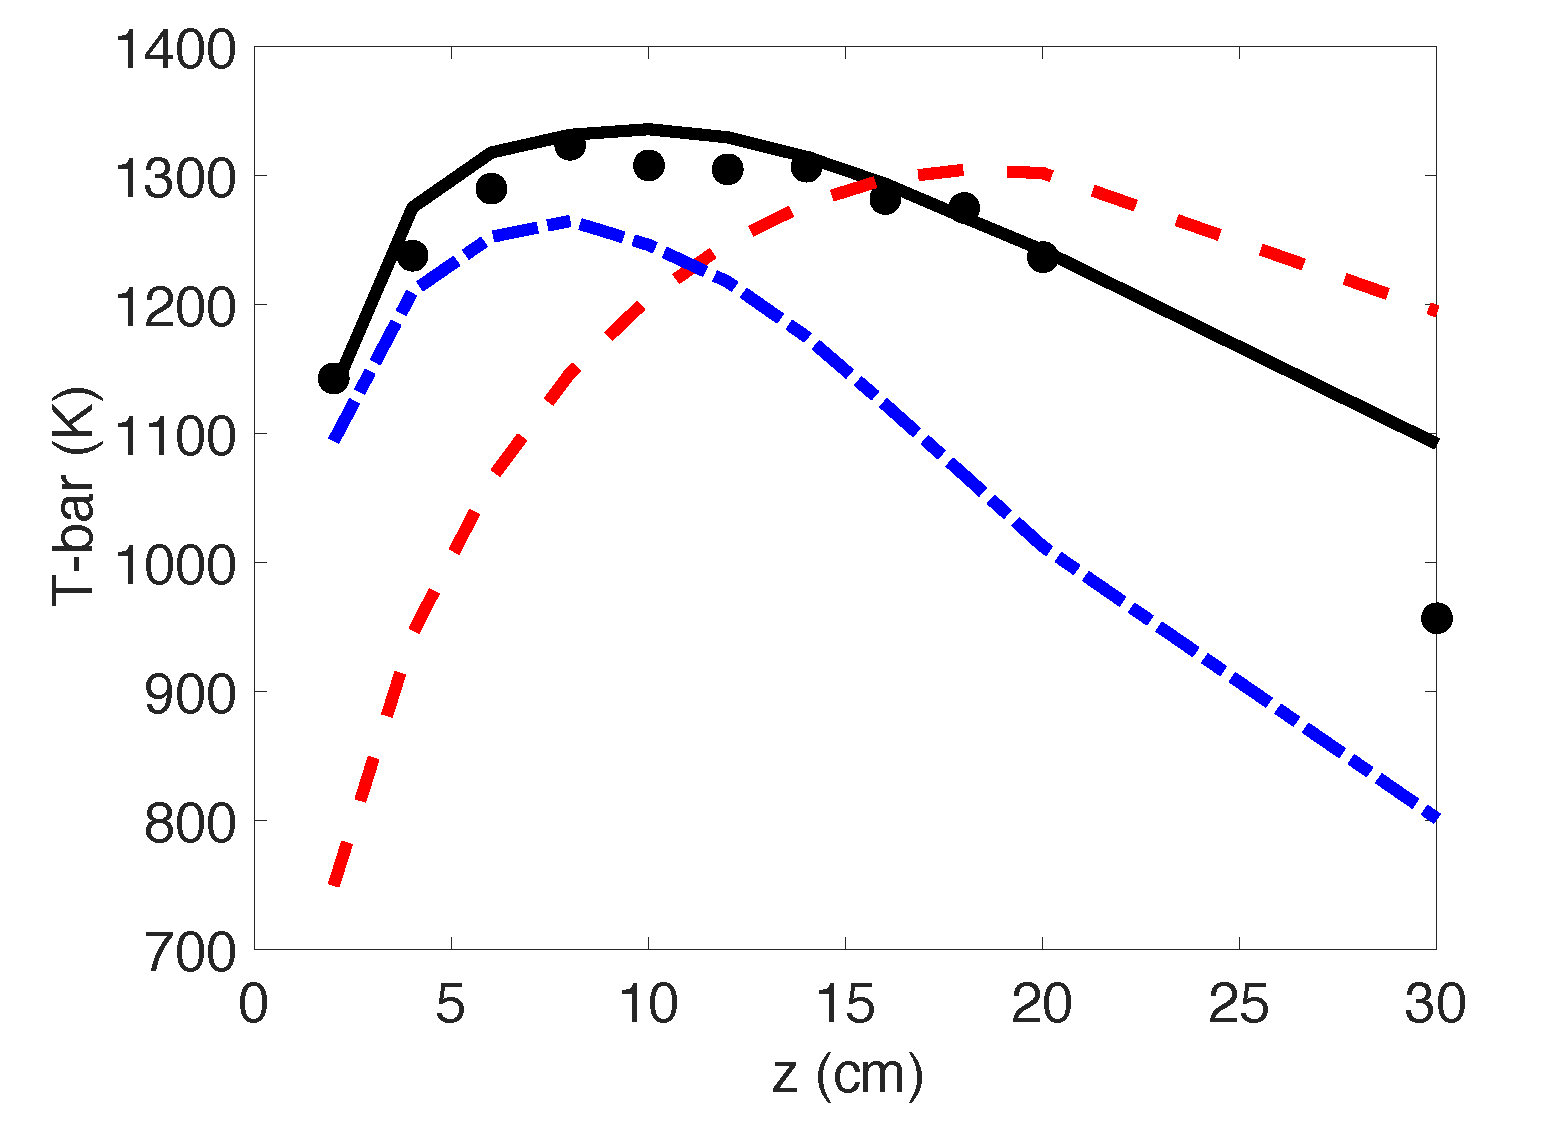
\includegraphics[height=2.2in]{Figures/Case3-Fig1a.png}
(b)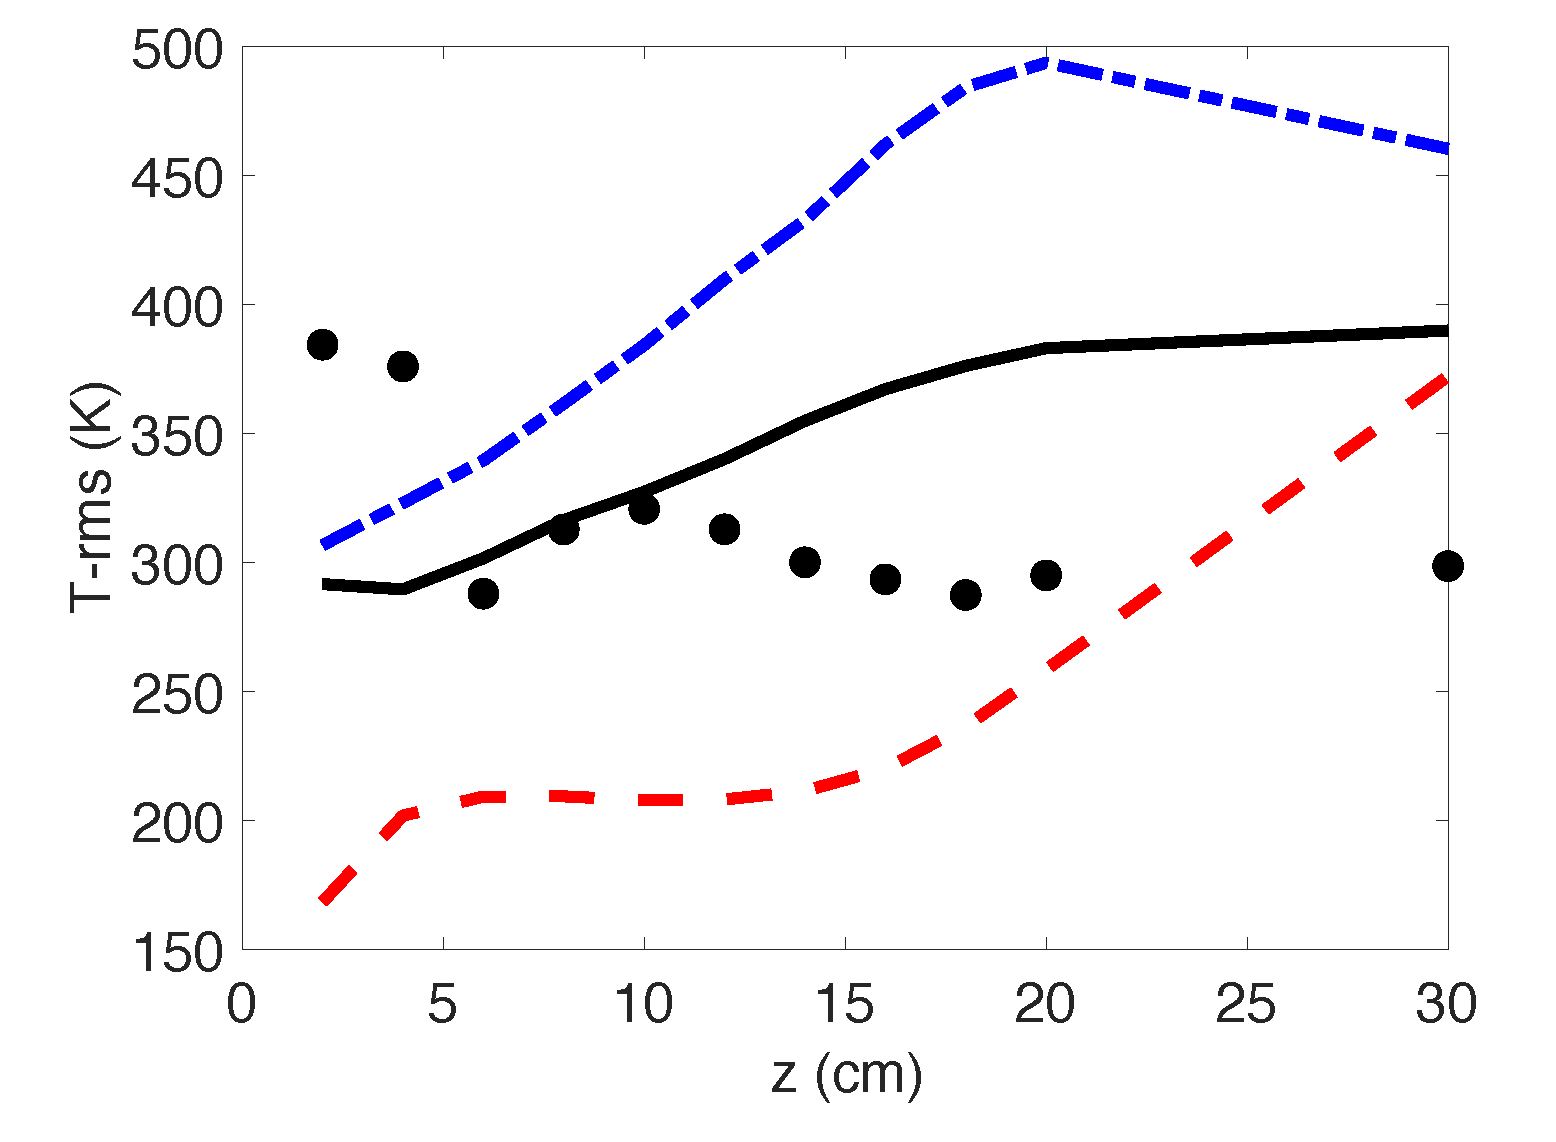
\includegraphics[height=2.2in]{Figures/Case3-Fig1b.png}
(c)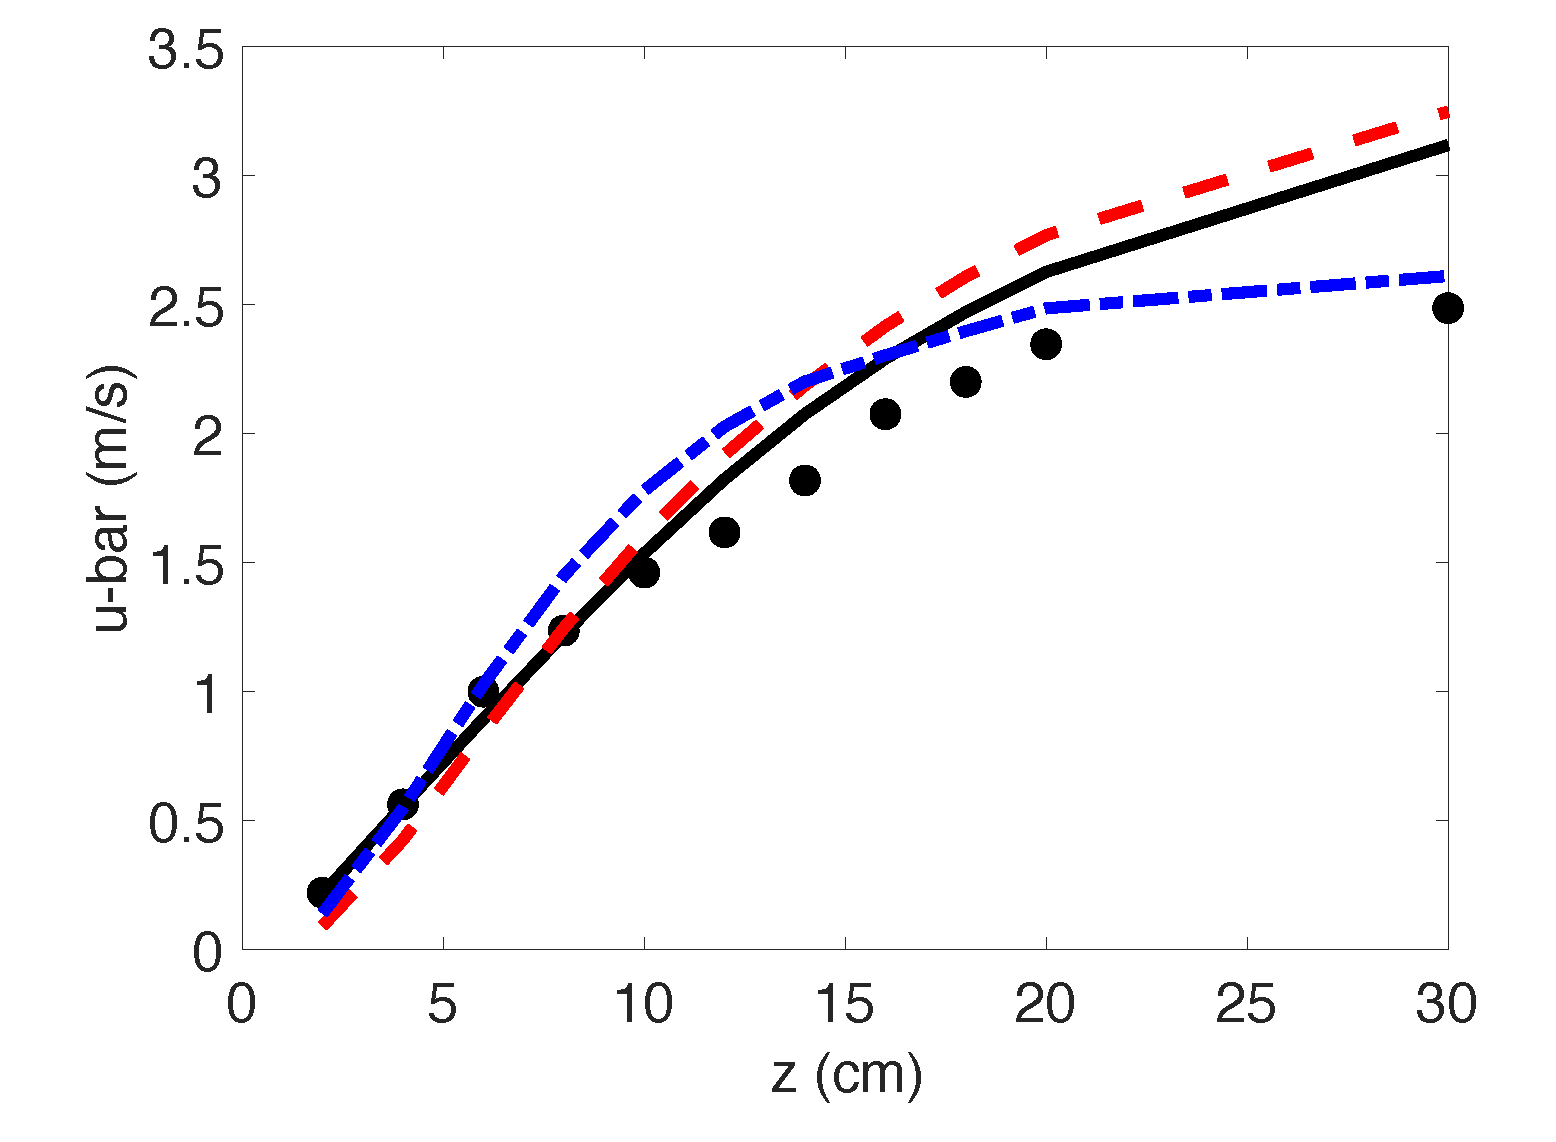
\includegraphics[height=2.2in]{Figures/Case3-Fig1c.png}
(d)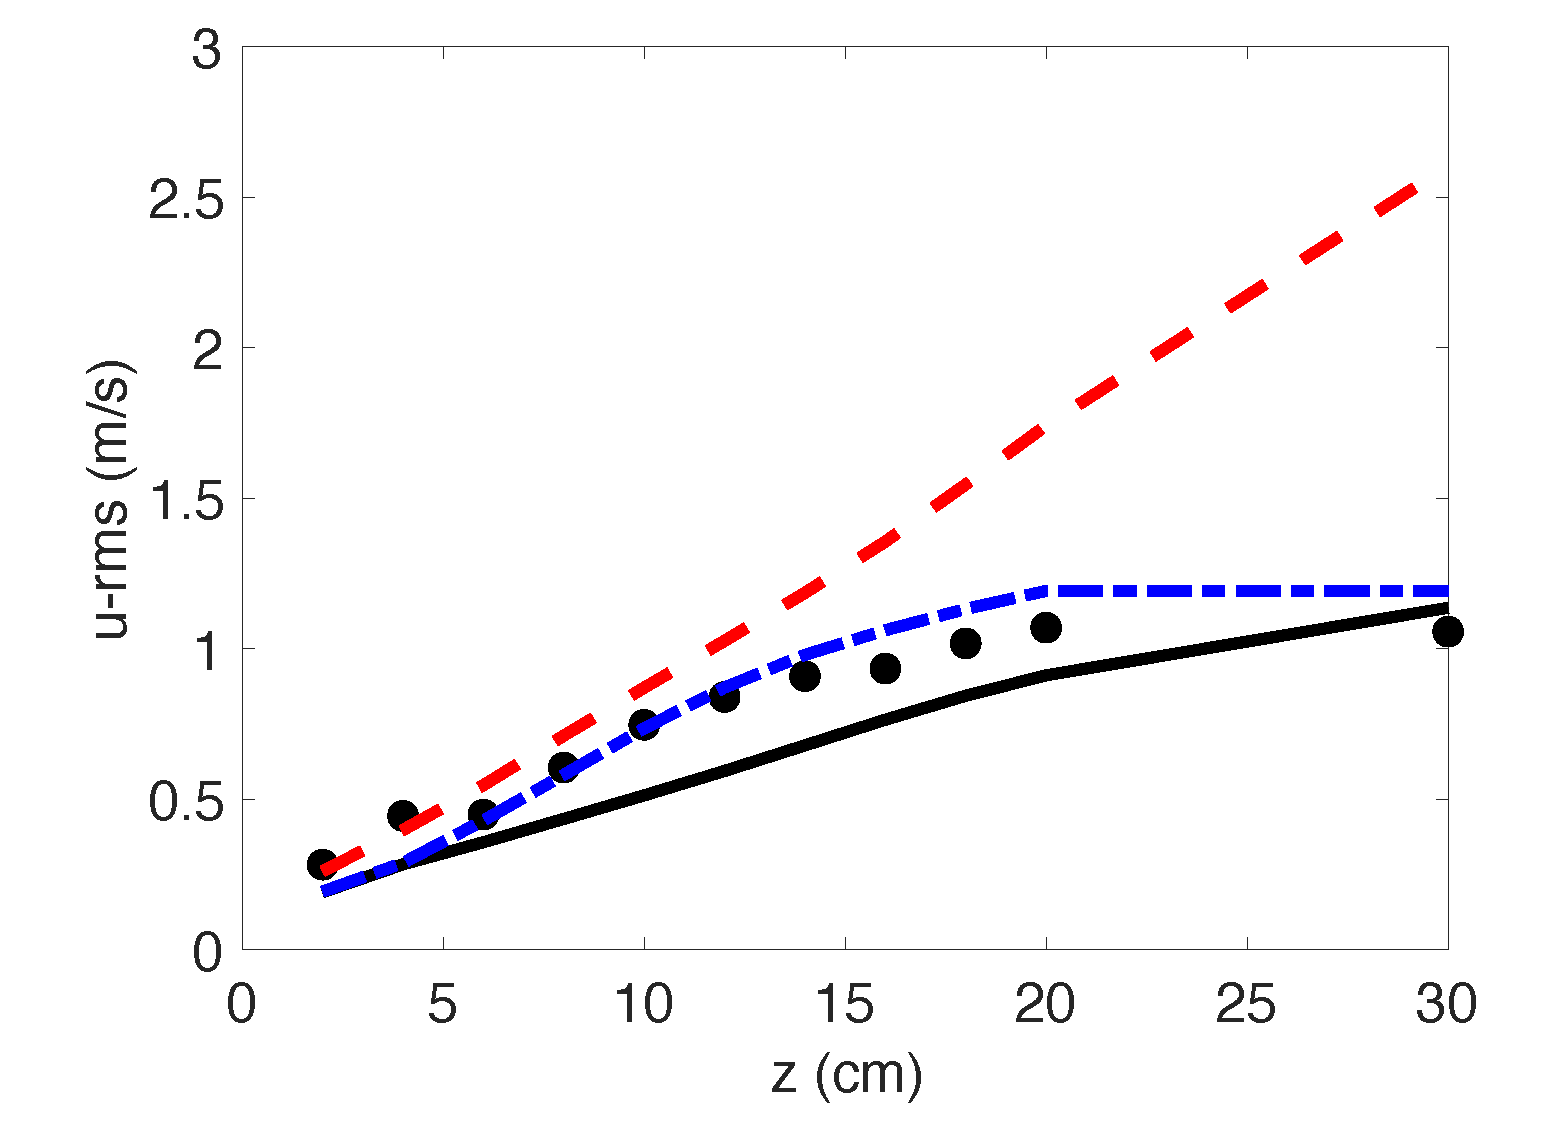
\includegraphics[height=2.2in]{Figures/Case3-Fig1d.png}
\caption{Case 3. Vertical variations along the pool centerline: (a) mean temperature; (b) {\it rms} temperature; (c) mean vertical velocity; (d) {\it rms} vertical velocity. Comparison between experimental data (black circles) and numerical results from UGent (black solid line), UMD (red dashed line), VTT (blue dash-dotted line).}
\label{fig:Case3-Fig1}
\end{figure}

Additional differences in the numerical treatment of the UW experiment include differences in the choice of physical models (see section~\ref{sec:PM} for details on baseline choices). UGent deviated from baseline choices in FireFOAM and used the dynamic Smagorinsky model~\cite{Moin:1991} for subgrid-scale turbulence, the Eddy Dissipation Concept (EDC) model~\cite{Magnussen:1981} for combustion, and an emission/absorption treatment of the RTE for radiation combined with a Weighted-Sum-of-Gray-Gases model~\cite{Dorigon:2013} for gas radiation (the global radiative loss fraction was predicted to be equal to 16.4\%, a value that is close to the empirically-determined value of 17-18\%); in the solution of the RTE, the discretization of angular space used 72 angles. UMD used the baseline configuration of FireFOAM; the value of the global radiative loss fraction was prescribed as equal to 18\%; in the solution of the RTE, the discretization of angular space used 16 angles. VTT used the baseline configuration of FDS: the values of the global radiative loss fraction was prescribed as equal to 17\%; in the solution of the RTE, the discretization of angular space used 104 angles.

\begin{figure}
\centering
(a)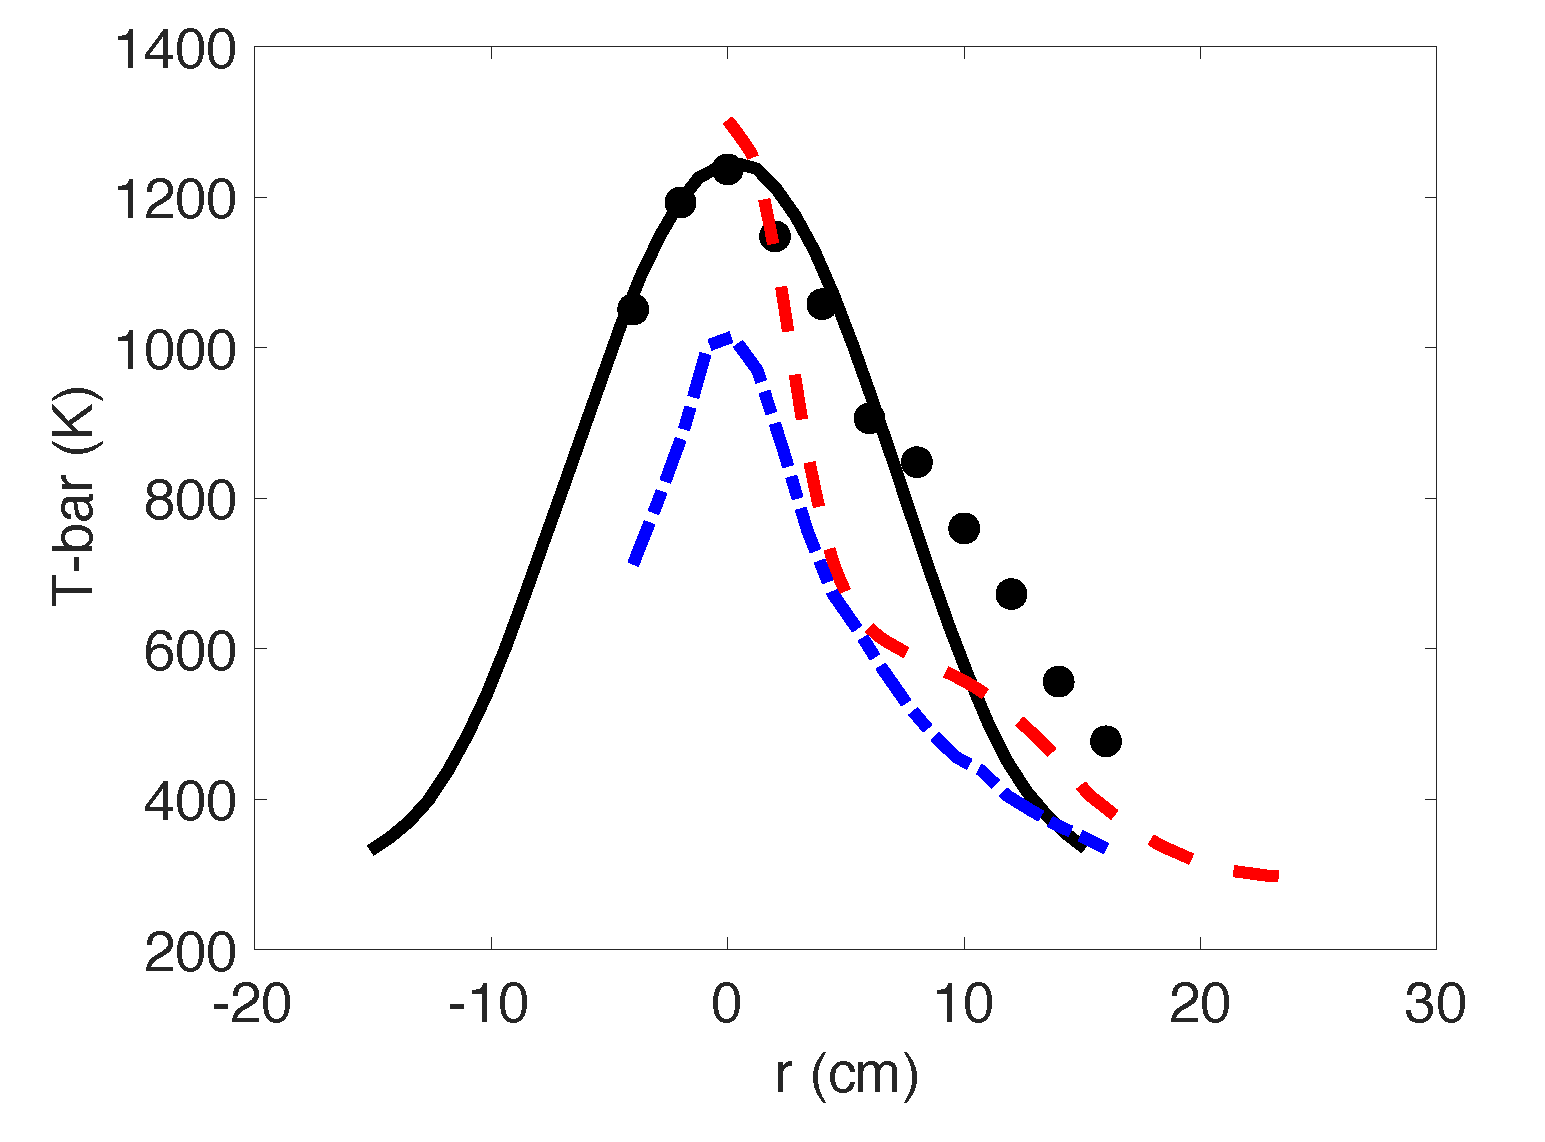
\includegraphics[height=2.2in]{Figures/Case3-Fig2a.png}
(b)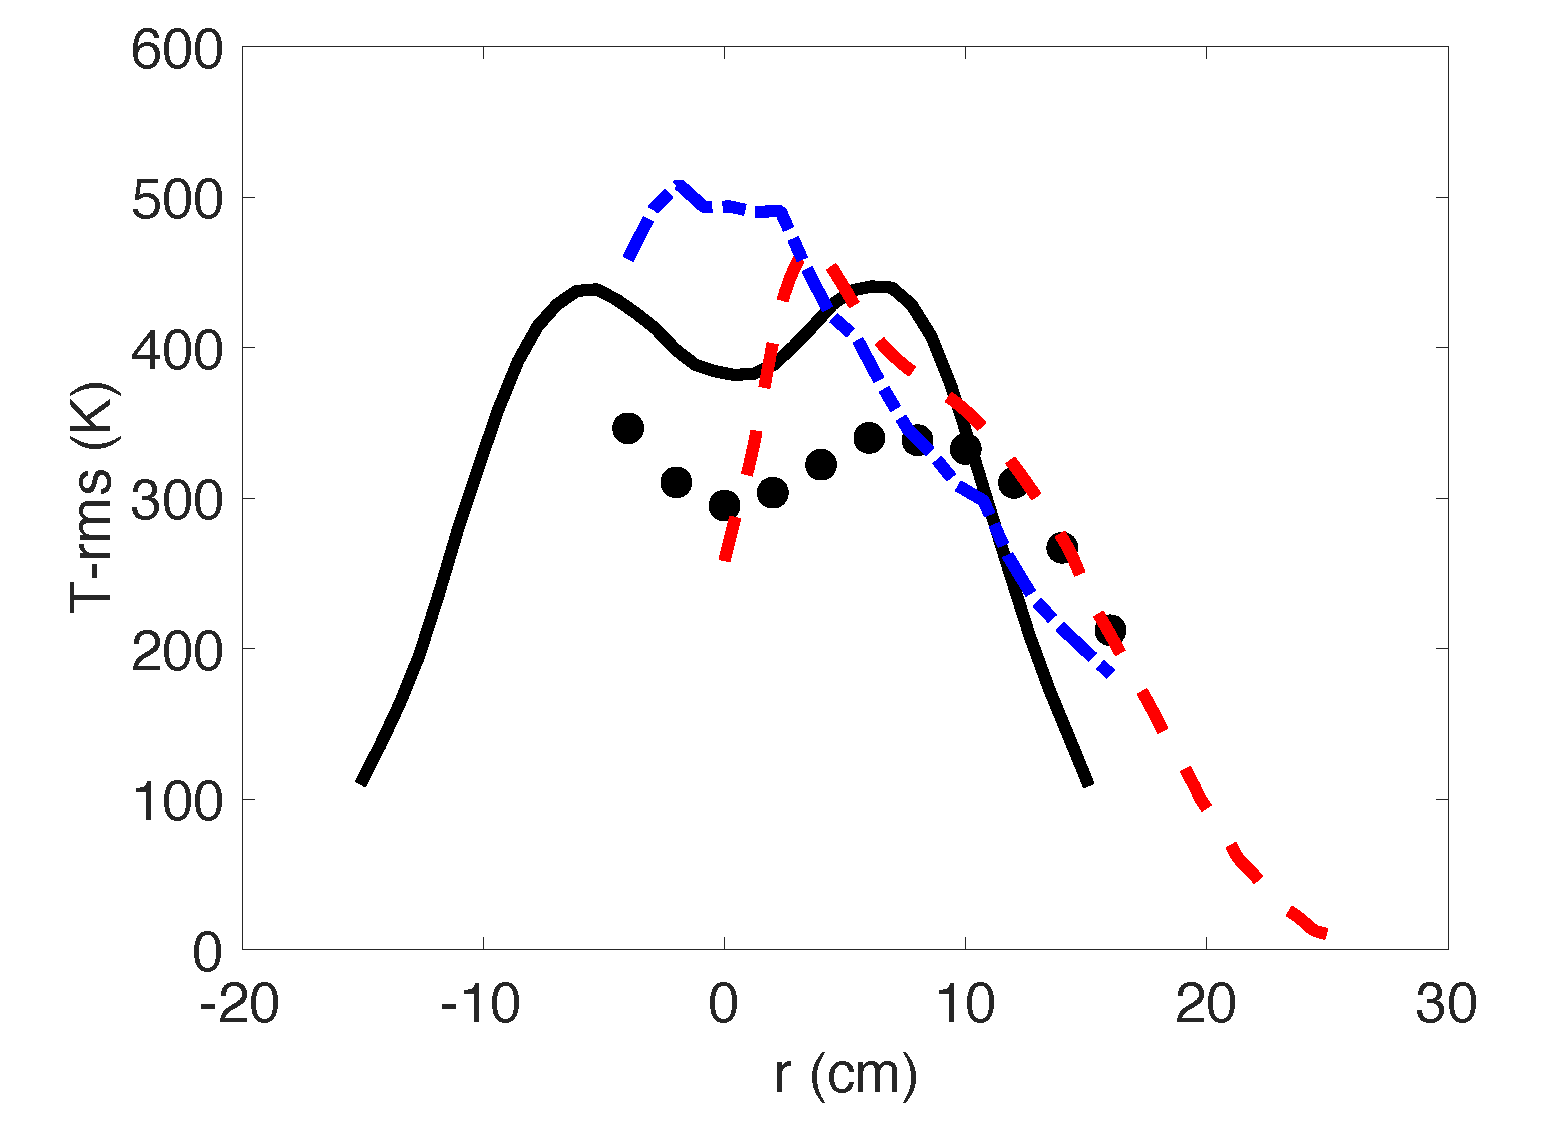
\includegraphics[height=2.2in]{Figures/Case3-Fig2b.png}
(c)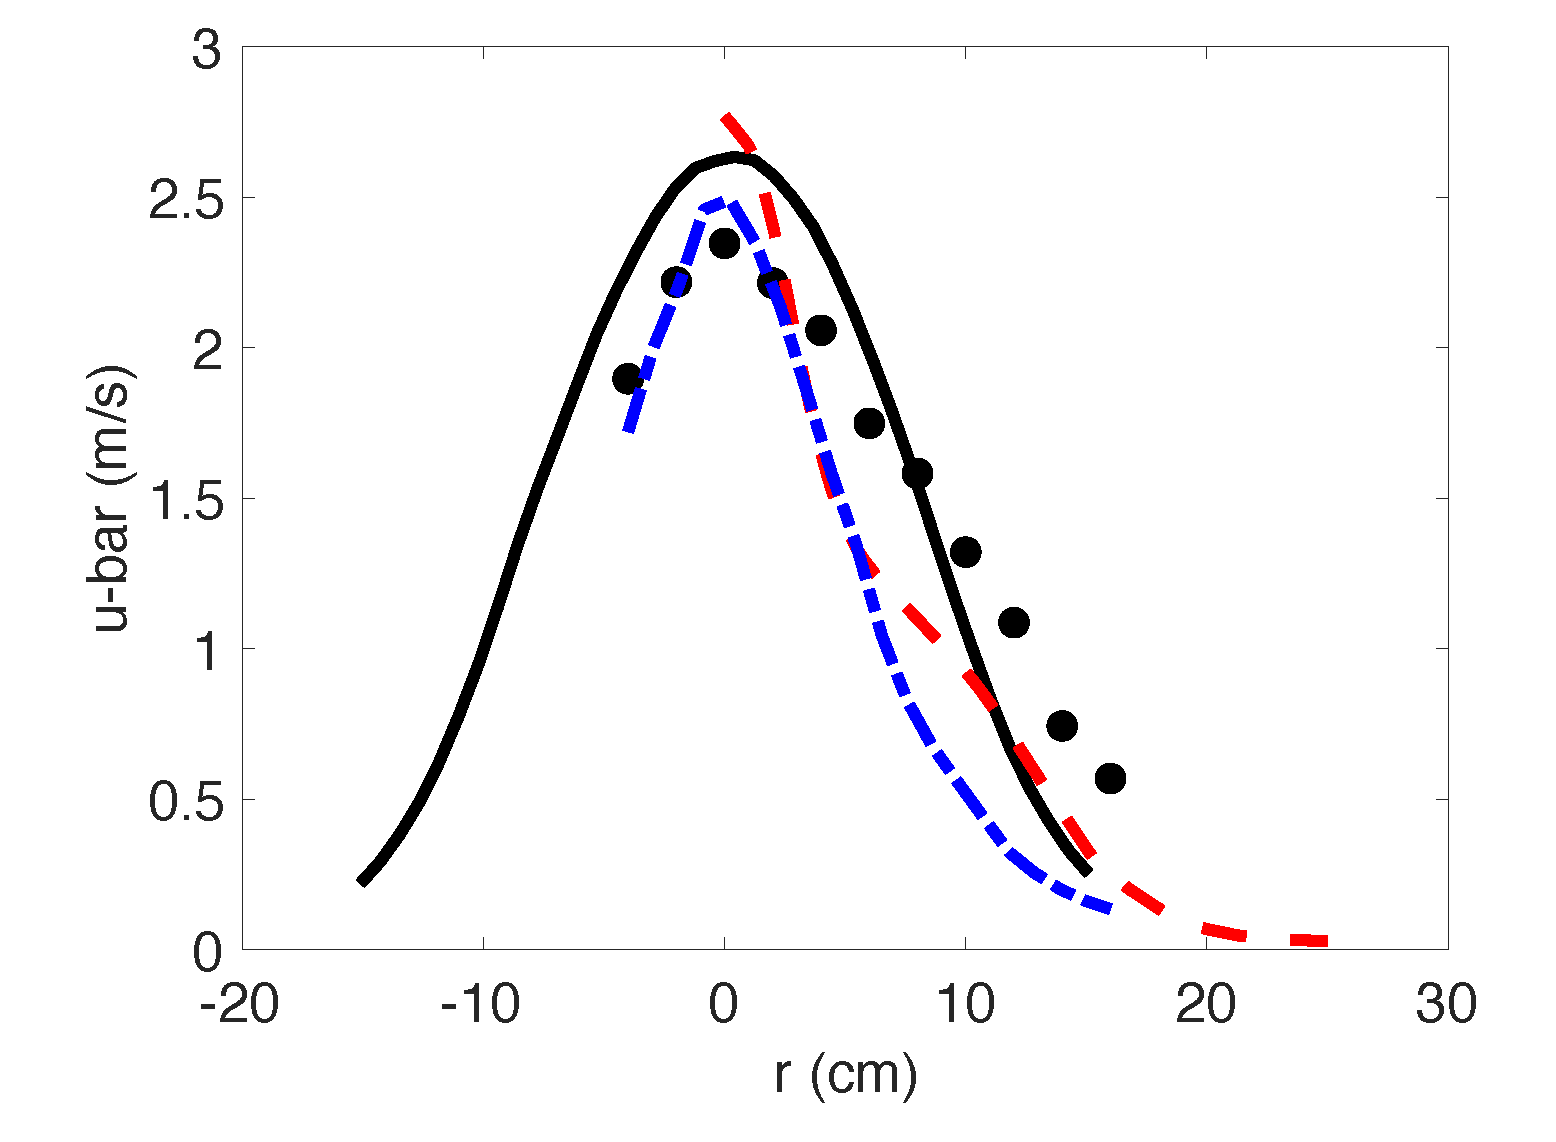
\includegraphics[height=2.2in]{Figures/Case3-Fig2c.png}
(d)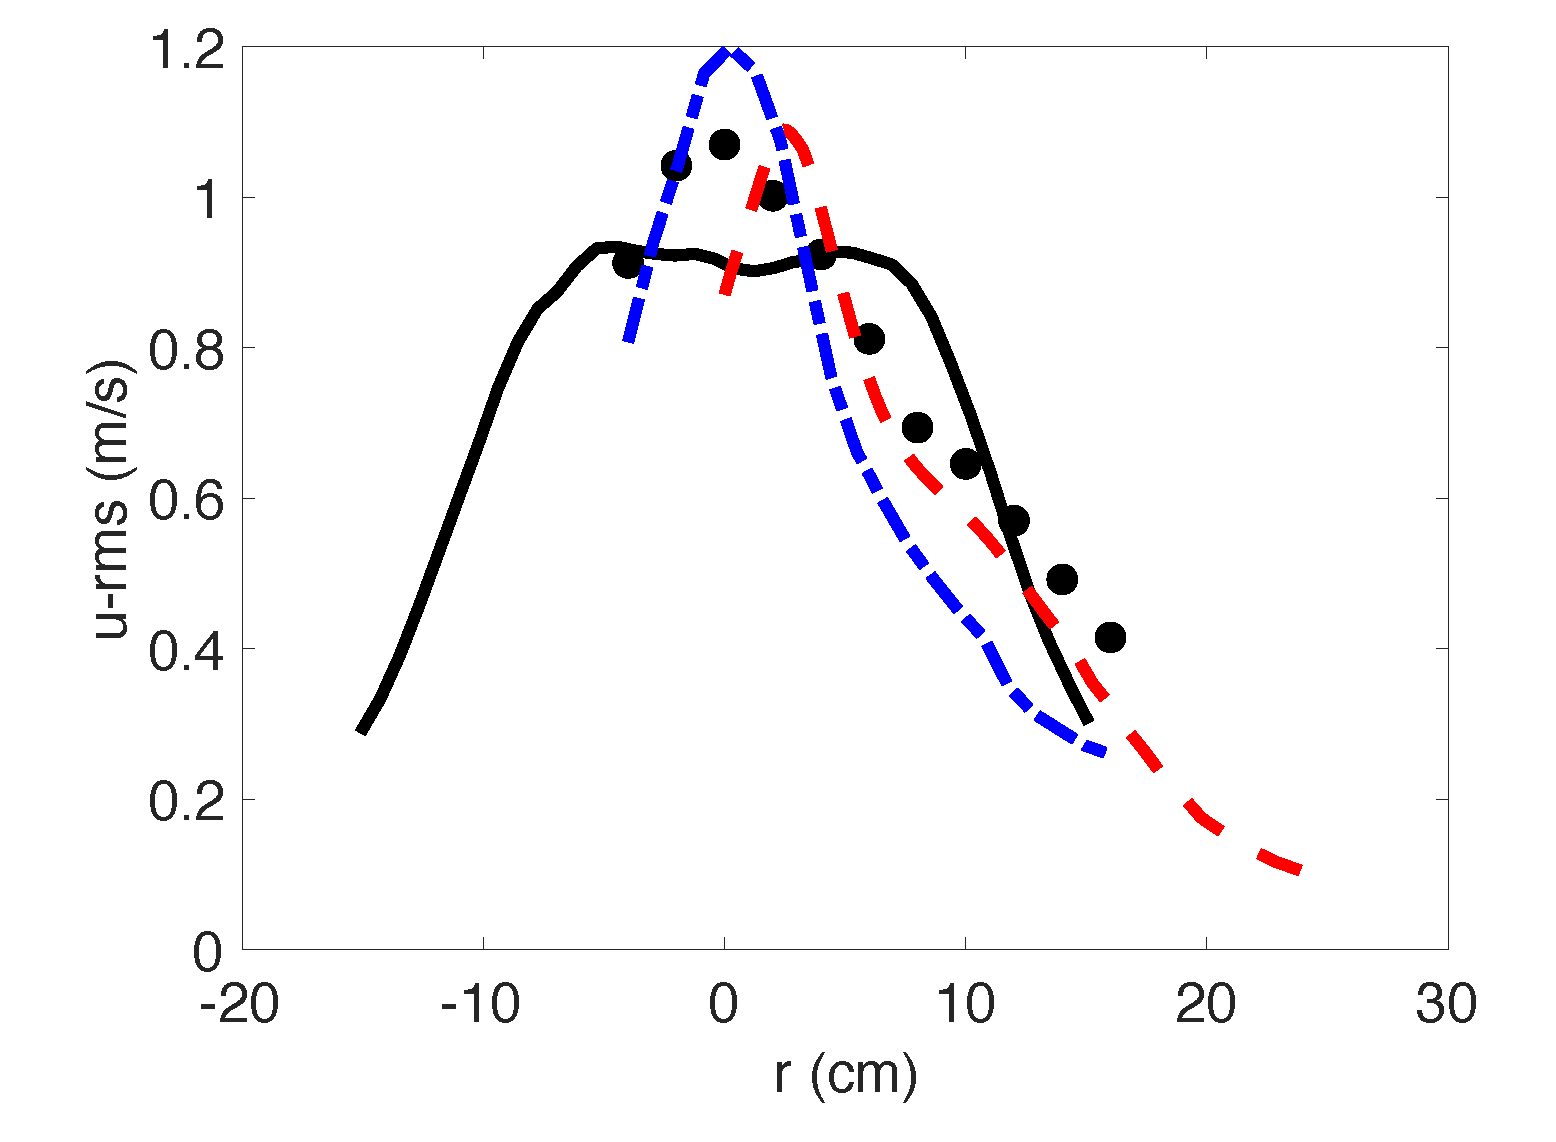
\includegraphics[height=2.2in]{Figures/Case3-Fig2d.png}
\caption{Case 3. Radial variations at elevation $z$ = 20~cm: (a) mean temperature; (b) {\it rms} temperature; (c) mean vertical velocity; (d) {\it rms} vertical velocity. See caption of Fig.~\ref{fig:Case3-Fig1}.}
\label{fig:Case3-Fig2}
\end{figure}

\subsubsection{Summary}

All simulations correctly reproduce a pulsating flame with a frequency of oscillation close to the measured value (2.8 Hz): 2.8 Hz (UGent), 2.2 Hz (UMD), 3 Hz (VTT). Figures~\ref{fig:Case3-Fig1} and~\ref{fig:Case3-Fig2} present a small representative sample of comparisons between experimental data and numerical simulations. Additional comparisons can be found in~\cite{MaCFP_wks_presentations}. Overall, the UGent simulation shows good agreement with experimental data and provides a satisfactory description of the flame structure. The accuracy of the UMD simulation is limited by insufficient grid resolution. The accuracy of the VTT simulation is limited by an inaccurate prediction of the total heat release rate.

It is worth emphasizing that the experimental database describing the UW methanol pool fire experiment is quite unique because it not only contains data on first and second-order statistical moments of temperature and vertical/radial velocities, but also contains data on Reynolds shear stresses and turbulent heat fluxes~\cite{Case3_EXP_1,Case3_EXP_2}. There are also some limitations in the database that are worth pointing out for future studies: (1) the UW database is limited to the flame near-field, $i.e.$ to low elevations ($z \leq 30$~cm), and there is a need to provide data over the full flame region ($0 \leq z \leq L_f$, where $L_f$ is the flame height; $L_f  \approx 0.5$~m in the UW experiment); (2) the flame is only weakly turbulent and there is a need to provide data for larger flame sizes, $i.e.$ for larger pool diameters ($D \geq 1$~m); (3) the thermal feedback is not characterized and there is a need to provide data on the convective/radiative heat flux at the liquid fuel surface.






% !TEX root = macfp_2017_gasphase.tex

\subsection{Case 4: Turbulent Wall Fires} \label{sec:wall_fires}

\subsubsection{Experiment}

Turbulent fire on a vertical surface is a canonical configuration representing the upward flame spread problem, typical in many practical fire scenarios. The FM Global vertical wall flame experiment selected for the first MaCFP workshop~\cite{Case4_EXP_1,Case4_EXP_2} is a series of meter-scale wall fires (the total heat release rate is several 100s of kW) realized by an array of vertically-stacked water-cooled porous gas burners with prescribed fuel supply rates. The setup conveniently decouples the gas-phase fire dynamics and corresponding heat transfer from the solid-phase pyrolysis, and thereby achieves a statistically steady-state condition ideal for experimental measurements and CFD model validation. The original goal of the experiment was to provide data to establish theoretical models and correlations for radiative and convective gas-to-solid heat transfer in wall fires. The fuel type and the fuel injection rate were varied in the tests. The total flame-to-wall heat flux as well as inward and outward flame radiation intensities were measured at different elevations. Other measurements included wall-normal profiles of gas temperature and flow velocity and vertical profiles of the soot depth. This experimental configuration provides MaCFP with the following: a canonical configuration that brings data on flame-wall interactions with realistic scales and buoyant turbulent flow conditions; a simplified statistically-stationary configuration that brings data on the different forms of heat transfer; and decoupled solid- and gas-phase processes through controlled fuel injection.

\subsubsection{Simulations}

Two groups submitted computational results for Case 4: FM Global~\cite{Case4_SIM_FMG} and NIST~\cite{Case4_SIM_NIST}. FM Global used FireFOAM version 2.2.x~\cite{FireFOAM}; NIST used an official release of FDS (version 6.5.3)~\cite{FDS}.

As discussed in section~\ref{sec:CGD}, the main challenge found in the design of a computational grid for LES simulations of the FM Global vertical wall flame experiment is to provide suitable grid resolution to capture the thin turbulent boundary layer flame. This requires millimeter-scale resolution. FM Global and NIST responded to this challenge in a similar way and adopted a 3-mm resolution in the near-wall flame region. In a previous study of the same wall fire configuration~\cite{Ren:2016}, this level of spatial resolution was found to be adequate for grid-resolved LES simulations ($i.e.$ for simulations that capture the wall gradients and are performed without using wall models). NIST chose to apply the 3-mm resolution in all directions and across the entire computational domain. FM Global chose a lower-cost computational grid and applied the 3-mm resolution in the wall-normal direction while using a 7.5-mm resolution in the spanwise and vertical directions (parallel to the wall) and also used a coarser mesh in the far field.

Additional differences in the numerical treatment of the wall flame experiment include differences in the choice of physical models (see section~\ref{sec:PM} for details on baseline choices). FM Global used the baseline configuration of FireFOAM except for using the WALE model~\cite{Ducros:1999} for subgrid-scale turbulence and for correct behavior in the near-wall region; the values of the global radiative loss fraction were prescribed using the measured values (to account for the radiation absorption from the fuel and cold soot in the near wall region, the prescribed values were chosen as 75\% of the values of the radiative loss fraction measured in corresponding wall-free configurations); in the solution of the RTE, the discretization of angular space used 16 angles. NIST used the baseline configuration of FDS except for using an emission/absorption treatment of the RTE based on a simplified soot formation model (using a prescribed soot yield) and a grey model for soot radiation as well as a wide-band (6 bands) model for gas radiation (with coefficients calibrated by the narrow-band model called RadCal~\cite{RadCal}); in the solution of the RTE, the discretization of angular space used 104 angles. Note that in its baseline configuration, FDS uses a Smagorinsky model with Van Driest wall functions~\cite{FDS_Math_Guide} to estimate a turbulent viscosity at the wall and a Nusselt-number-based convective heat transfer model to estimate the convective heat flux at the wall~\cite{FDS_Math_Guide}.

Interestingly, FM Global and NIST differ significantly in their near-wall treatment: while FM Global follows the modeling choices of Ref.~\cite{Ren:2016} and adopts a wall-resolved approach in which the wall convective heat flux is calculated by direct differentiation of the resolved temperature field (no wall model is used), NIST adopts a wall-modeled approach in which the wall convective heat flux is reconstructed by wall functions and Nusselt-number correlations. It is not clear whether the wall-modeled approach adopted by NIST converges towards a wall-resolved approach in case of sufficient grid resolution.

\begin{figure}
\centering
(a)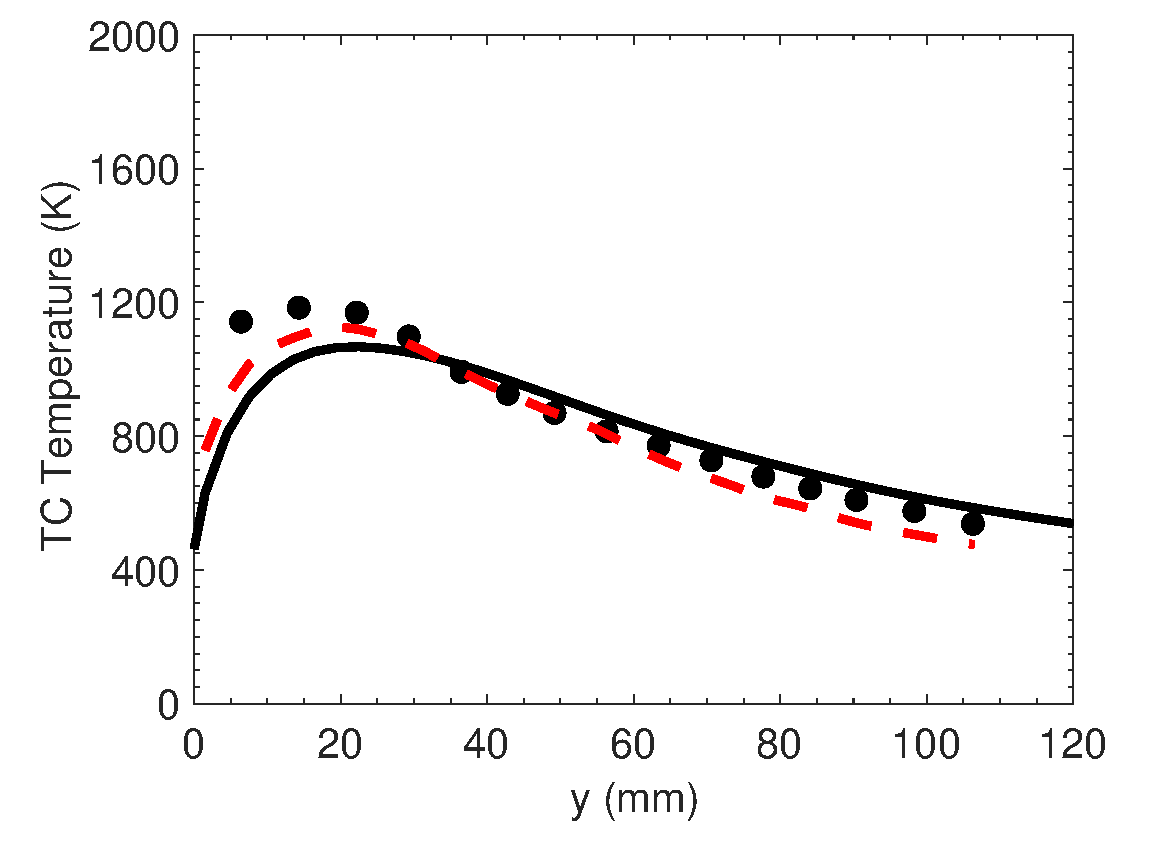
\includegraphics[height=2.2in]{Figures/Case4-Fig1a.pdf}
(b)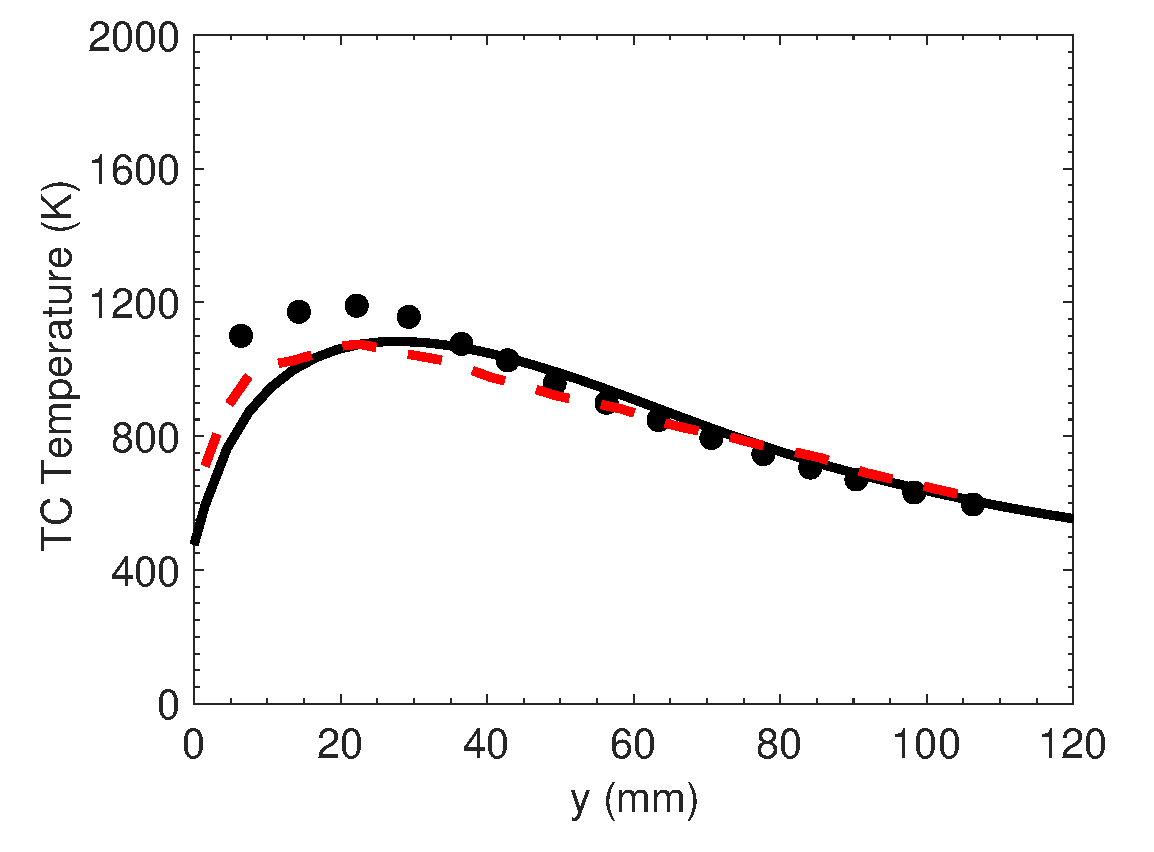
\includegraphics[height=2.2in]{Figures/Case4-Fig1b.pdf}
\caption{Case 4. Wall-normal variations of mean thermocouple temperature at $z$ = 0.77~cm and for a fuel supply rate equal to: (a) 12.68 g/m$^2/$s; (b) 17.05 g/m$^2/$s. Comparison between experimental data (black circles) and numerical results from FM Global (black solid line) and NIST (red dashed line). Case of a propylene flame.}
\label{fig:Case4-Fig1}
\end{figure}

\subsubsection{Summary}

We limit our discussion to the case of propylene fuel (additional results can be found in~\cite{MaCFP_wks_presentations}). Both FM Global and NIST simulations qualitatively reproduce the variations of the wall heat flux with vertical elevation as well as the variations of the wall heat flux in response to changes in the fuel supply rate. Figure~\ref{fig:Case4-Fig1} presents a representative sample of comparisons between measured and simulated thermocouple temperatures (note that in these comparisons, both FM Global and NIST simulations use a thermocouple model that is integrated inside the solvers and that uses the LES solution to simulate the deviations of thermocouple temperatures from gas temperatures). Figure~\ref{fig:Case4-Fig2} presents a sample of comparisons between measured and simulated wall heat fluxes. The NIST simulations overpredict the total heat flux by approximately 50\% in most scenarios. In contrast, the FM Global simulations shows good agreement with experimental data, a result that may be attributed to the choice of using a semi-empirical radiation model with an experimentally-determined global radiative loss fraction. These results suggest that even with a fine computational grid, a radiation treatment based on a simplified soot formation model combined with a grey model for soot radiation and a wide-band model for gas radiation is not sufficiently accurate to predict wall heat fluxes in a wall flame configuration. Note that because the experimental database does not include information on the convective and radiative components of the wall heat flux, this information was not extracted from the simulations. Future simulations of this case should analyze these components (see for instance Ref.~\cite{Ren:2016}) and also bring information on the relative weight of soot radiation and gas radiation.

\begin{figure}
\centering
(a)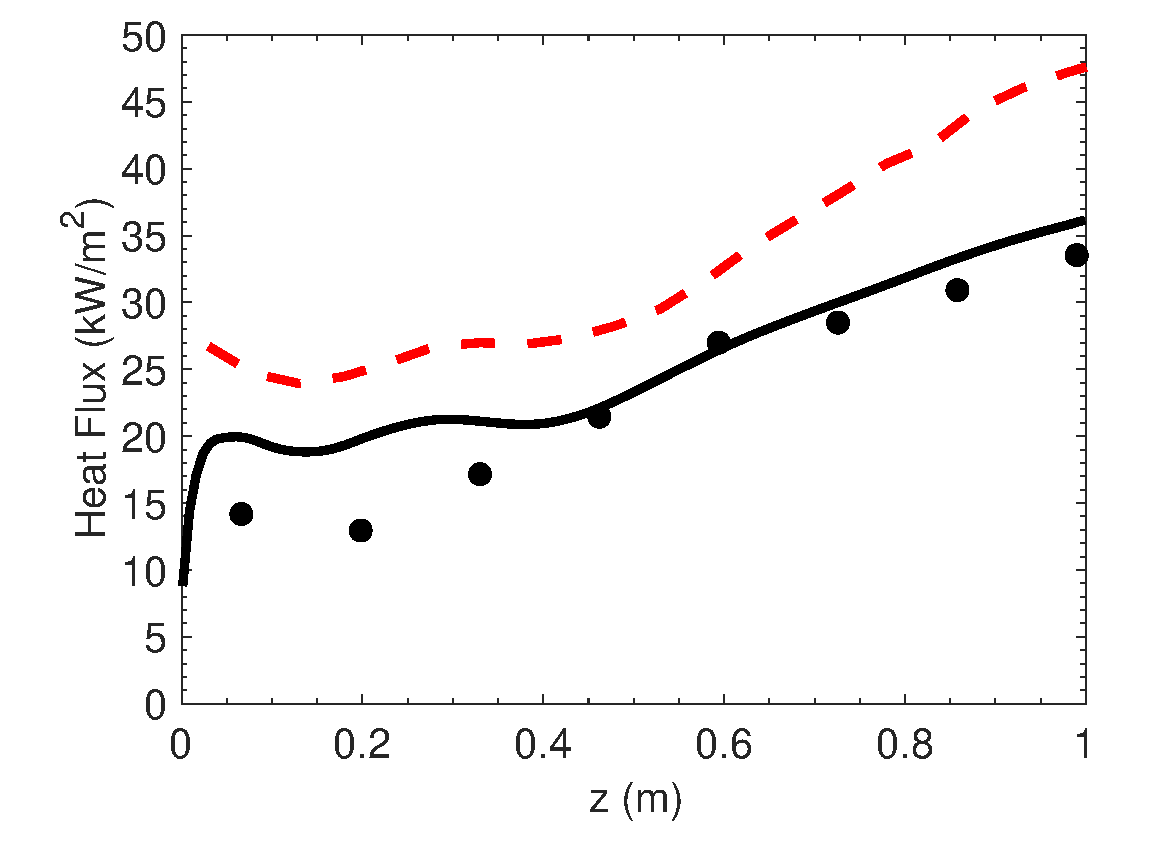
\includegraphics[height=2.2in]{Figures/Case4-Fig2a.pdf}
(b)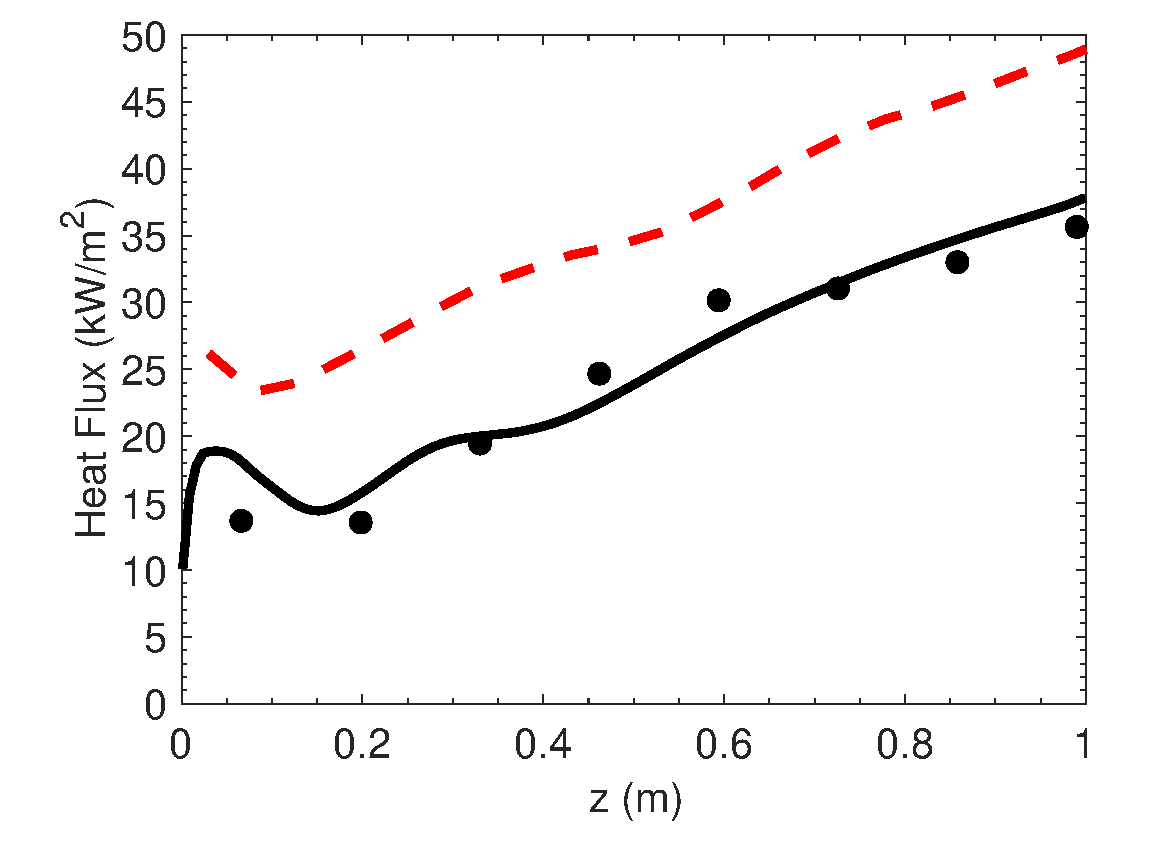
\includegraphics[height=2.2in]{Figures/Case4-Fig2b.pdf}
\caption{Case 4. Vertical variations of the mean total wall heat flux for a fuel supply rate equal to: (a) 12.68 g/m$^2/$s; (b) 17.05 g/m$^2/$s. See caption of Fig.~\ref{fig:Case4-Fig1}.}
\label{fig:Case4-Fig2}
\end{figure}

In closing, the experimental database describing the FM Global vertical wall flame experiment is quite unique because it brings fundamental information on gas-to-solid heat transfer processes that are a controlling factor in flame spread problems. There are also some limitations in the database that are worth pointing out for future studies: (1) the database is limited to temporal means and does not contain information on fluctuation magnitudes; (2) the thermal feedback is characterized in terms of a total wall heat flux but does not contain information on the convective and radiative components of the wall heat flux, nor on the soot and gas contributions to the radiative component of the wall heat flux.

Furthermore, as already pointed out in section~\ref{sec:gaseous_pool_fires}, it is worth noting that while research-level simulations may accept the computational cost associated with millimeter-scale resolution, engineering-level simulations will not accept that cost and will use coarser grids that require wall models. The development and evaluation of these models is part of the future objectives of MaCFP.




% !TEX root = macfp_2017_gasphase.tex

\subsection{Case 5: Flame Extinction} \label{sec:flame_extinction}

\begin{figure}
\centering
(a)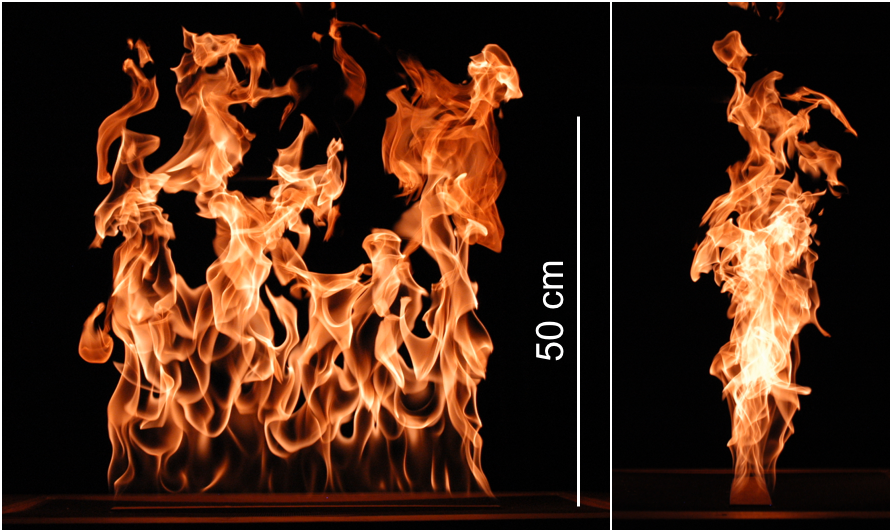
\includegraphics[height=1.3in]{Figures/Case5-Fig1a.png}
(b)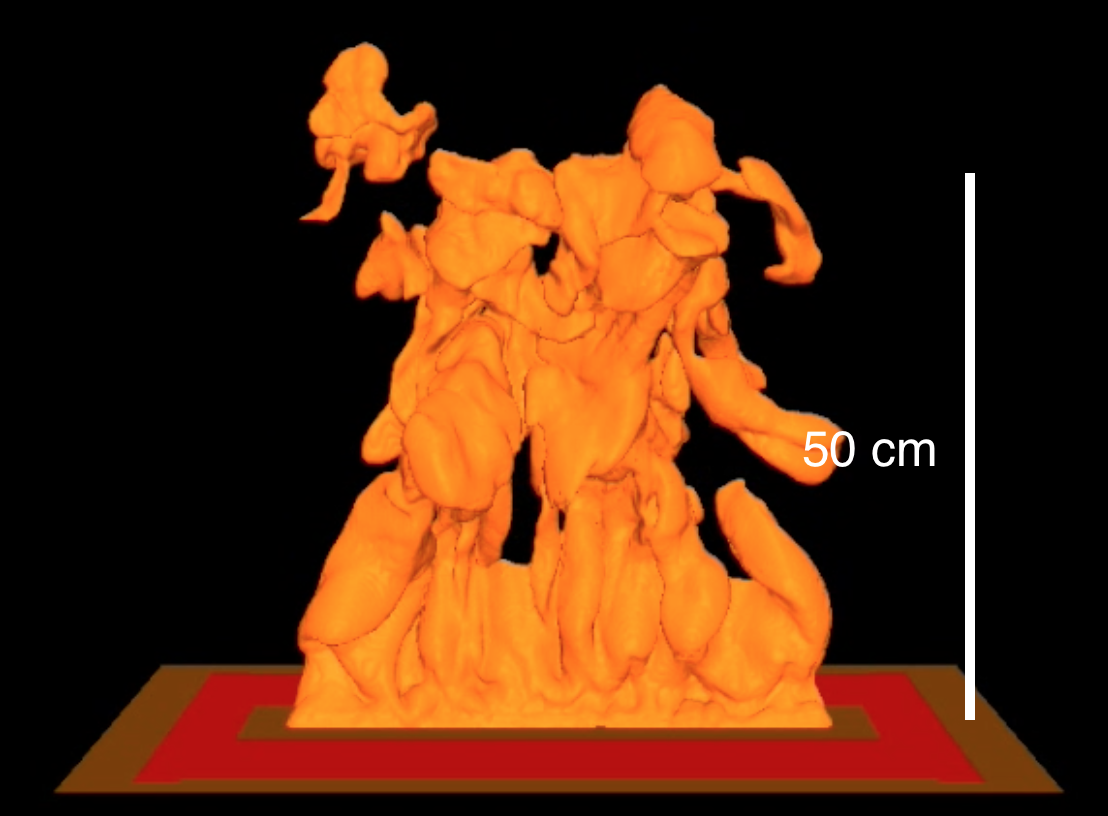
\includegraphics[height=1.3in]{Figures/Case5-Fig1b.png}
(c)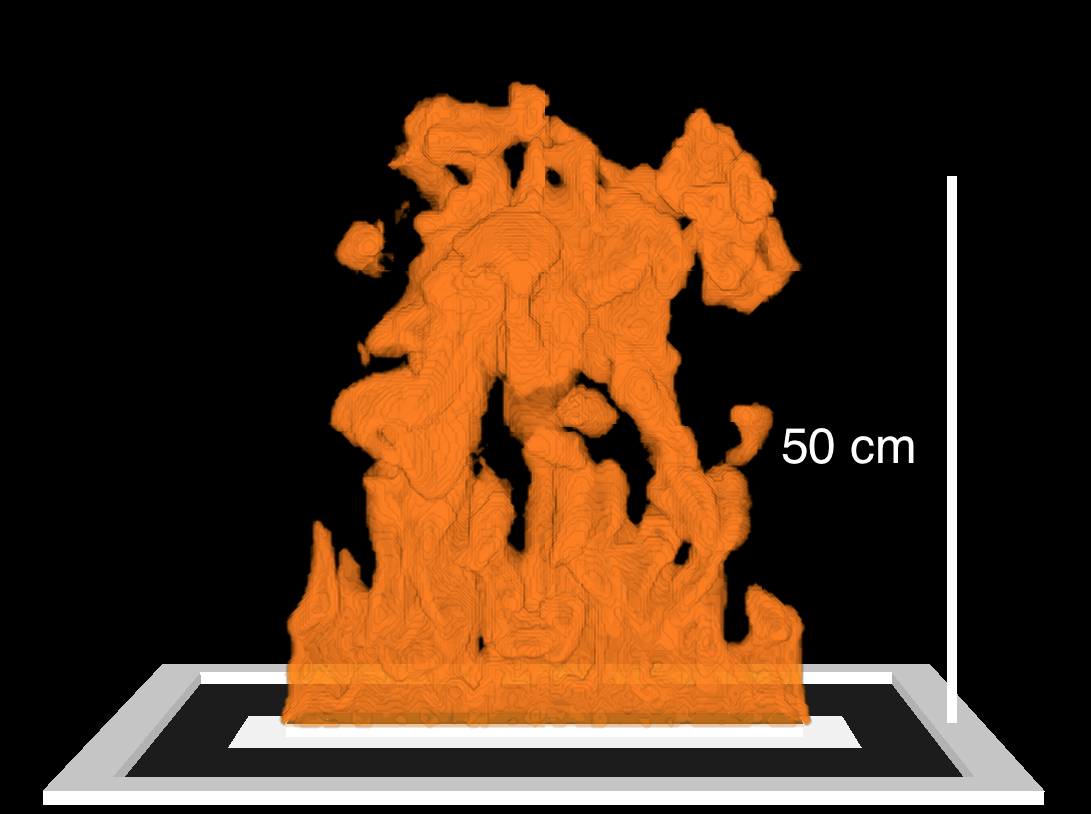
\includegraphics[height=1.3in]{Figures/Case5-Fig1c.png}
\caption{Case 5. Instantaneous snapshot of the methane-air flame in the UMD turbulent line flame experiment: (a) experiment (both front and side view); (b) FireFOAM simulation (front view); (c) FDS simulation (front view). In all figures, the vertical white line indicates 50~cm elevation.}
\label{fig:Case5-Fig1}
\end{figure}

\subsubsection{Experiment}

The flame extinction experiment selected for the first MaCFP workshop is a canonical line-fire configuration with controlled co-flow studied at the University of Maryland (UMD)~\cite{Case5_EXP_1,Case5_EXP_2,Case5_EXP_3}. The UMD turbulent line burner facility allows the study of a buoyancy-driven, turbulent diffusion flame exposed to environments of decreasing oxygen strength, down to the oxygen extinction limit, and thereby provides fundamental information relevant to fire suppression due to under-ventilation or due to the activation of an inert gas system. The facility comprises a sand-filled, stainless-steel fuel port, slot burner, 5-cm-wide and 50-cm-long. Controlled suppression of the flame is achieved via the introduction of nitrogen gas into the co-flowing oxidizer stream.

Both methane and propane fuels were utilized. Assuming complete combustion, the total heat-release rate was 50~kW for both fuels (the flame was approximately 0.5~m-high). The quantitative metric of suppression is the global combustion efficiency, $\eta$, reported as a function of the coflow oxygen strength and measured using oxygen consumption and carbon dioxide generation calorimetry~\cite{Case5_EXP_3}. The mole fraction of oxygen, $X_{\text{O}_2}$, was measured using a paramagnetic oxygen analyzer via a probe located inside the oxidizer port. Infrared radiative emissions were measured using a water-cooled Schmidt-Boelter heat-flux transducer; heat flux data were then converted to global radiative loss fractions using a weighted multipoint radiation source model~\cite{Case5_EXP_2}. Visible flame height was measured using a video camera. A limited set of temperature measurements is also available for methane fuel and $X_{\text{O}_2} = 18 \%$.

\begin{figure}
\centering
(a)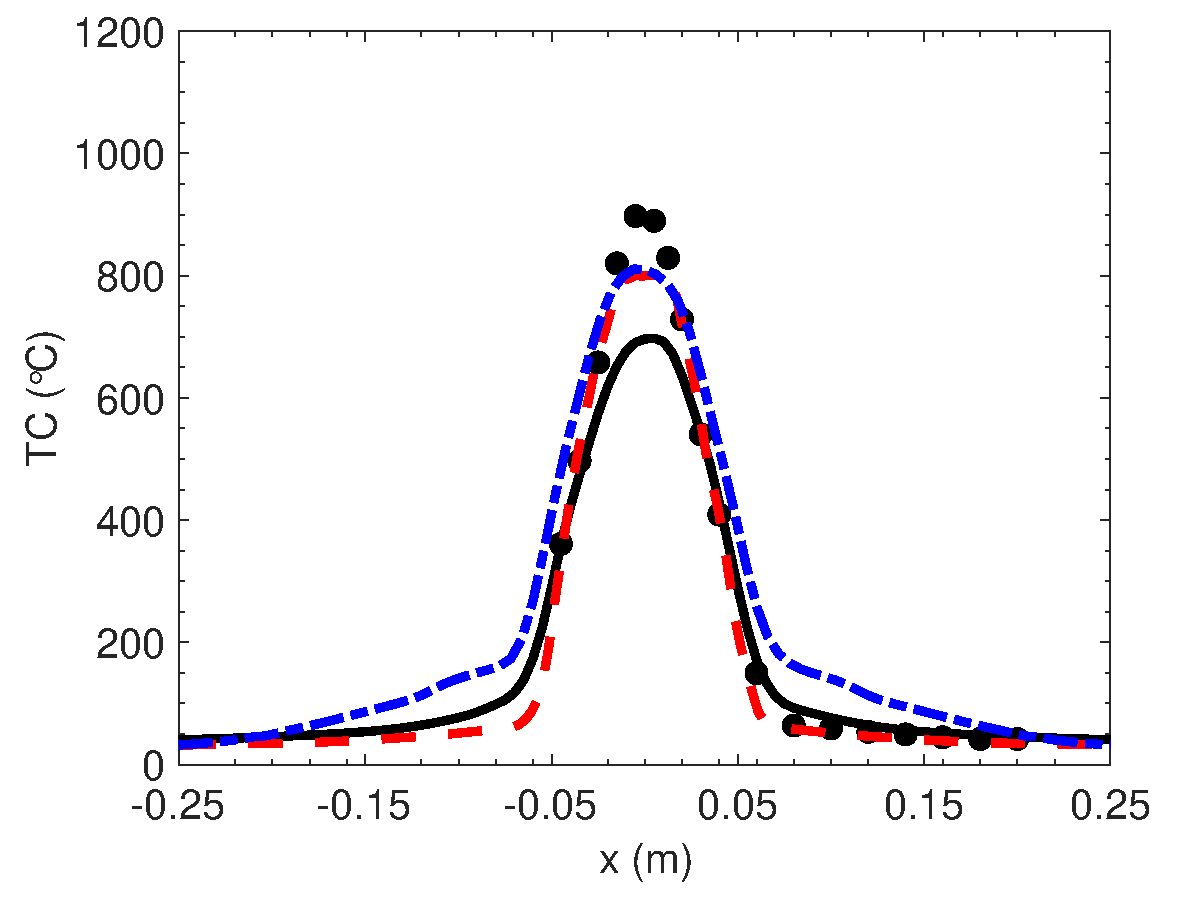
\includegraphics[height=2.2in]{Figures/Case5-Fig2a.pdf}
(b)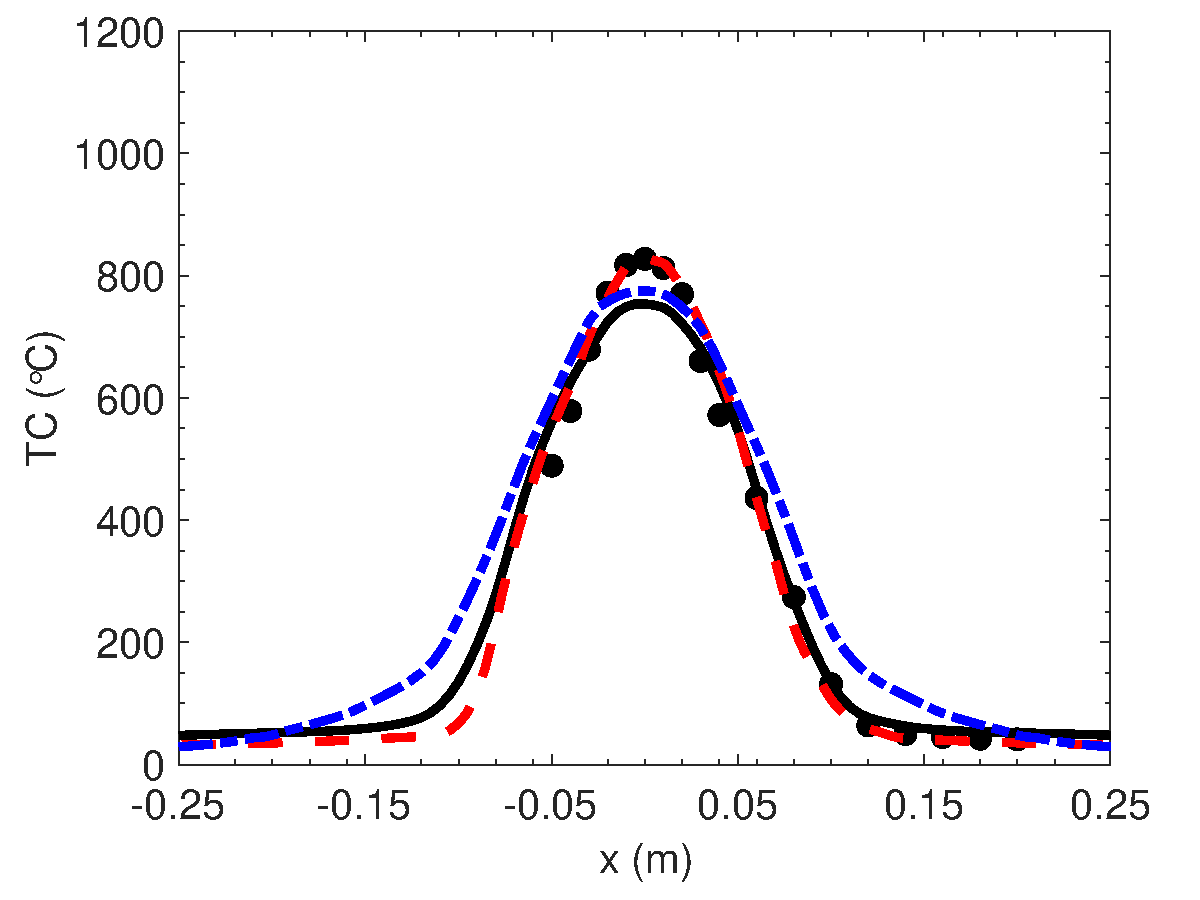
\includegraphics[height=2.2in]{Figures/Case5-Fig2b.pdf}
\caption{Case 5. Cross-flame variations of mean thermocouple temperature at: (a) $z = 0.125$ m; (b) $z = 0.25$ m. Comparison between experimental data (black circles) and numerical results from FM Global (black solid line), NIST (red dashed line), UMD (blue dash-dotted line). Case of a methane flame with $X_{O_2} = 18\%$. 
\label{fig:Case5-Fig2}}
\end{figure}

\subsubsection{Simulations}

Three groups submitted computational results for Case 5: FM Global~\cite{Case5_SIM_FMG}, NIST~\cite{Case5_SIM_NIST} and UMD~\cite{Case5_SIM_UMD}. FM Global and UMD used a shared development version of FireFOAM (FireFOAM-dev)~\cite{FireFOAM}; NIST used an official release of FDS (version 6.5.3)~\cite{FDS}.

As discussed in section~\ref{sec:CGD}, the main challenge found in the design of a computational grid for LES simulations of the UMD turbulent line flame experiment is to provide suitable grid resolution to capture the controlling length scale of the burner, $i.e.$ the burner width (5~cm). This requires millimeter-scale resolution. The computational groups responded to this challenge in a similar way and adopted a resolution of 5-mm (FM Global), 3.125-mm (NIST) and 4.2~mm (UMD) in the flame region.

Additional differences in the numerical treatment of the line flame experiment include differences in the choice of physical models (see section~\ref{sec:PM} for details on baseline choices). FM Global and UMD used the baseline configuration of FireFOAM except for the addition of a flame extinction model based on the concept of a critical Damk\"ohler number for premixed eddies~\cite{Dorofeev:2016} (FM Global) or the concept of a critical Damk\"ohler number for diffusion flames~\cite{Vilfayeau:2016} (UMD); the values of the global radiative loss fraction were prescribed using the measured values~\cite{Case5_EXP_2}; in the solution of the RTE, the discretization of angular space used 16 angles. NIST used the baseline configuration of FDS except for the addition of a flame extinction model based on the concept of a critical flame temperature~\cite{Vaari:2011,White:2017}; in the solution of the RTE, the discretization of angular space used 700 angles (the large number of angles is due to the fact that the NIST simulation included the heat flux gauge located at 1-m distance from the flame and was motivated by the desire to avoid any potential ray effect). 

\begin{figure}
\centering
(a)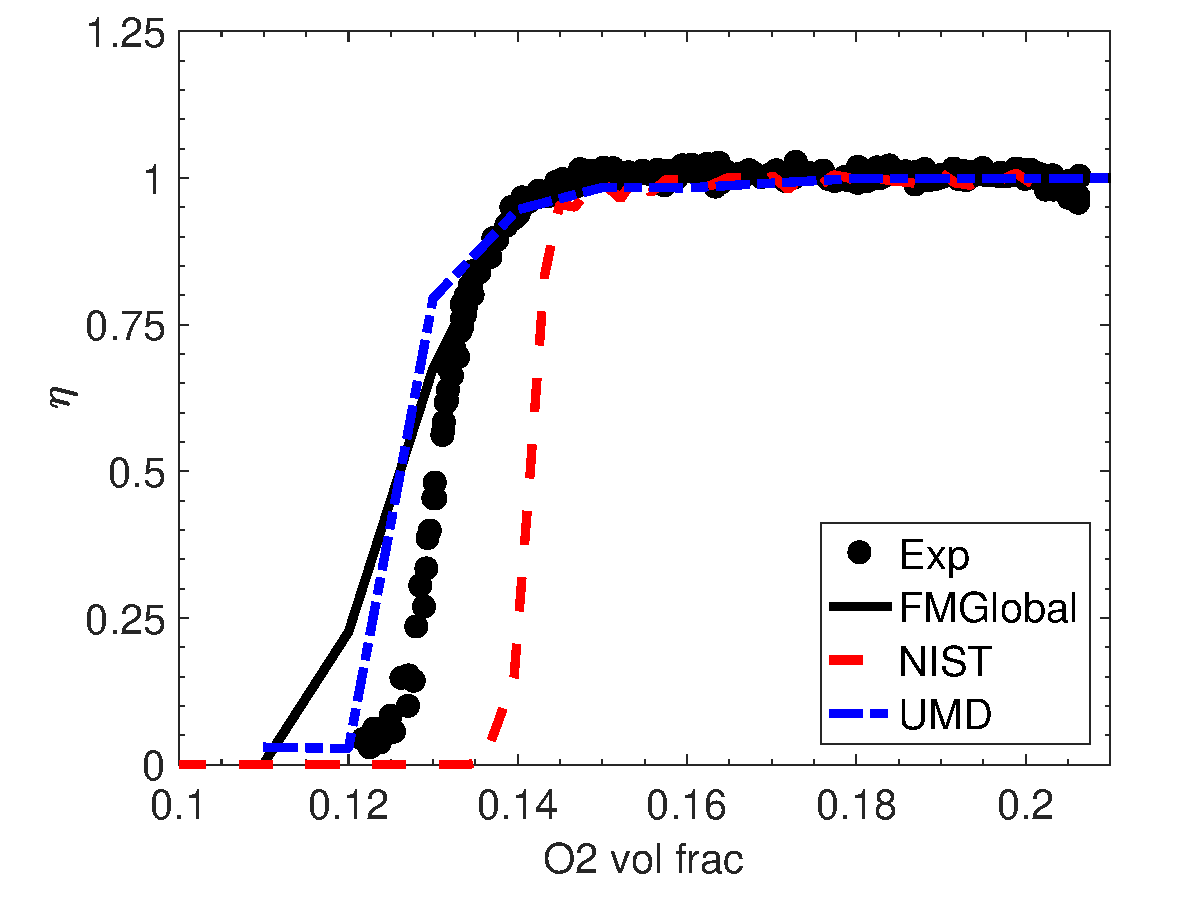
\includegraphics[height=2.2in]{Figures/Case5-Fig3a.pdf}
(b)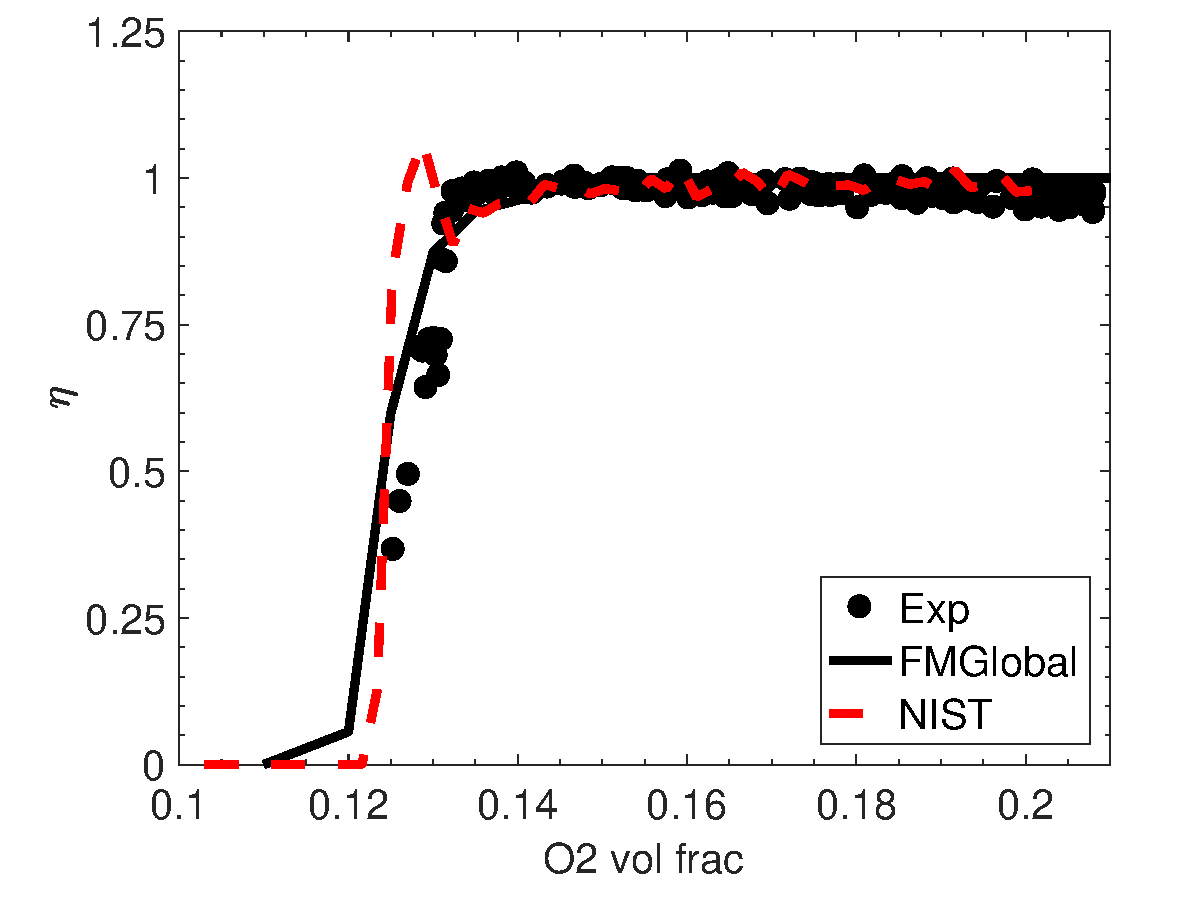
\includegraphics[height=2.2in]{Figures/Case5-Fig3b.pdf}
\caption{Case 5. Variations of the global combustion efficiency with the coflow oxygen mole fraction. (a) methane flame; (b) propane flame. See caption of Fig.~\ref{fig:Case5-Fig2}.}
\label{fig:Case5-Fig3}
\end{figure}

\subsubsection{Summary}

All simulations seem to reproduce the overall structure of the turbulent flame (see Fig.~\ref{fig:Case5-Fig1}.). Figure~\ref{fig:Case5-Fig2} presents comparisons between measured and simulated thermocouple temperatures performed at quarter-flame height and at mid-flame height (note that in these comparisons, all simulations use a thermocouple model). Figure~\ref{fig:Case5-Fig2} suggests that the level of agreement between experimental data and numerical results is encouraging; discrepancies are however observed, especially at quarter-flame height, and those may be attributed to inaccuracies in the combustion model, in the thermal radiation model, or in the coupling of these models.

Figure~\ref{fig:Case5-Fig3} presents comparisons between measured and simulated combustion efficiencies as a function of the coflow oxygen strength,  for both methane and propane flames. All simulations correctly reproduce the binary nature of the flame response: the combustion efficiency remains close to 1 for $X_{\text{O}_2}$ above the extinction limit and abruptly decreases to 0 at this limit ($i.e.$ for $X_{O_2} \approx$ 12-14 \%). The exact value of the oxygen extinction limit is predicted within $\pm$ 10-20\%. While these results are encouraging, it is worth emphasizing that the flame extinction models are complex (they in fact rely on a description of both extinction and re-ignition phenomena~\cite{Dorofeev:2016,Vilfayeau:2016,White:2017}) and that the models used in the FM Global, NIST and UMD simulations are based on different representations of the physics. Thus, the UMD turbulent line flame database is not capable of differentiating between the three flame extinction models and therefore does not provide sufficient insight into the underlying physics of flame suppression. Also, as mentioned in section~\ref{sec:CGD}, it is important to recognize that the FM Global and UMD flame extinction models (and to a lesser extent the NIST flame extinction model) were originally tuned against data obtained from the same UMD experiment. Therefore, the simulations should be interpreted as \emph{calibration} tests rather than validation tests.

Note that the UMD turbulent line flame database has been recently enhanced with new micro-thermocouple measurements and has also been extended to the case of flame suppression by a water mist~\cite{Case5_EXP_1}. These new developments should be incorporated into MaCFP. The addition of micro-thermocouple measurements will provide much needed data to characterize the details of the flame structure (and will provide both first- and second-order statistics). More information on flow velocity as well as on gas and soot radiation will also be needed in order to unravel the respective effects of combustion and thermal radiation.













% !TEX root = macfp_2017_gasphase.tex

\subsection{Current and Future Plans} \label{sec:plans}

The gas phase session of the June-2017 MaCFP workshop provided a first opportunity to demonstrate the benefits and potential impact of activities organized by the IAFSS MaCFP Working Group. The session provided a community-wide forum for in-depth technical discussions of a first suite of experimental-computational comparisons corresponding to an initial list of target experiments. The session was well attended (with 120 registered participants) and the first general lesson from the workshop is that MaCFP successfully responds to a need for greater levels of integration and coordination in fire research. The fire science community is small, fragmented and geographically dispersed: MaCFP is an effort to meet the resulting organizational challenge, to build an international collaborative framework, and to provide a critical mass of researchers for topics central to the development of a fundamental understanding of fire phenomena. While MaCFP is currently focused on building a collaborative framework between computational and experimental researchers around the topic of the validation of CFD-based fire models, we envision that MaCFP can be extended to incorporate efforts focused on other topics, or can be emulated and inspire other efforts.

The gas phase session of the first MaCFP workshop also led to a number of technical lessons and outcomes that will help shape the future activities of MaCFP. First, as discussed in section~\ref{sec:cfd_review}, the performance of CFD-based fire models depends on both the quality of the computational grid (and in particular its ability to resolve the dynamically-controlling length scales of the simulated problem) and the accuracy of the physical models (used to describe subgrid-scale turbulence, combustion, radiation, {\it etc}). In this context, it is important to emphasize that the submissions made by the seven different computational groups represented at the MaCFP workshop correspond to fine grid resolution at the millimeter- or centimeter-scale. Under high-resolution simulation conditions, the impact of numerical errors is reduced and many of the discrepancies between experimental data and computational results may be attributed to modeling errors. While fine-grained simulations are considered as a necessary step, and provide valuable insights into the accuracy of physical models, they are not representative of engineering-level simulations that typically use coarser grids: there is therefore an unmet need for MaCFP to also evaluate physical models in coarse-grained simulations that are more representative of the CFD practice. This will be addressed in future editions of the MaCFP workshop series. Note that one objective of the MaCFP Working Group is to develop guidelines for CFD practitioners for the design of the computational grid as well as reference material on the domain of validity of the different physical models available in current CFD-based fire models.

Furthermore, discussions of the different target experiments revealed a number of limitations in available experimental databases that are worth pointing out for future studies: (1) the databases are often limited to small-scale, weakly-to-moderately turbulent flames and there is a need to provide more data for large-scale fully-developed turbulent flames; (2) the databases are often limited to measuring temporal means and there is a need to provide data on fluctuation magnitudes; (3) the databases are often limited to the flame near-field and there is a need to provide data over the full flame region; and (4) the databases are often focused on characterizing the flow field or the temperature field, but not both, and there is a need to provide more comprehensive data sets including flow velocities, temperatures, and also soot volume fractions, radiation intensities and heat fluxes to surfaces. Note that the availability of quality data on radiation intensities and heat fluxes to surfaces is a requirement for future progress on simulations of flame spread phenomena. We hope that the wish list above will inspire a new generation of experimentalists and motivate new experimental studies.

Finally, as discussed in section~\ref{sec:intro}, the initial list of target experiments selected for the first MaCFP workshop had a limited scope corresponding to (mostly) non-sooting or only weakly-sooting flames, supplied with gaseous or liquid fuel, and without compartment effects. There is now a need to extend the scope of MaCFP to include target experiments that bring detailed information on a number of key fire processes, for instance: thermal radiation, soot formation and oxidation, flame spread along solid flammable materials (see the next section), and also ignition phenomena and compartment effects. In addition, the application of current fire models to the simulation of water-based fire suppression systems ($i.e.$ sprinkler or mist systems) requires additional experimental data and validation tests on water droplet dispersion, evaporation and radiation blockage. The intent of MaCFP is to expand the list of target experiments. It is also to keep re-visiting the initial list for further insights into basic flow and combustion phenomena and for additional tests with coarse-grained simulations. 

In closing, the organizing committee of the MaCFP Working Group has now started preliminary discussions for the organization of a second workshop. Interested individuals/organizations are encouraged to contact the committee~\cite{MaCFP_website} in order to join MaCFP, influence the selection of new target experiments, participate in discussions on the structure, format and scope of MaCFP, participate in discussions on the location and time of the second workshop. Note that the experimental and computational databases corresponding to Cases 1-5 are hosted on the MaCFP repository~\cite{MaCFP_repository} and are available to the fire research community as reference data for future experimental and/or computational studies. The MaCFP Working Group is committed to continuously update the repository.


\section{Condensed Phase Subgroup} \label{sec:CPS_session}

% !TEX root = macfp_2017_gasphase.tex

\subsection{Objectives} \label{sec:CPS_session_1}

The production of combustible gases by burning materials is typically the rate-limiting process in the growth of fire.  A quantitative understanding of this process is therefore essential for advancing our ability to predict and mitigate fire development.  Unfortunately, measurement and modeling efforts carried out in this field by various research groups tend to be poorly coordinated.  Little agreement exists as to what constitutes best practices and standards in data collection and model development.  The purpose of the condensed phase subgroup of the MaCFP Working Group is to facilitate data and model sharing among researchers in order to improve predictions of thermal decomposition and pyrolysis in fire.  The work of this subgroup, in conjunction with the work of the gas phase subgroup, is expected to lead to fundamental progress in fire modeling.  It is envisioned that the two subgroups will collaborate to make quantitative predictions of the combined gas-solid phase processes that determine flame spread.  It is also envisioned that the two subgroups will hold joint workshops every two or three years.

The condensed phase subgroup shares the central objective of MaCFP ``to target fundamental progress in fire science and to advance predictive fire modeling."  The specific objectives of the subgroup will focus on the development, calibration, verification, and validation of predictive models of thermal decomposition and pyrolysis.  To this end, the subgroup plans to:

\begin{itemize}
\item Develop several alternative formats for experimental data sets that carry sufficient information to enable parameterization of pyrolysis models for a given material.
\item Develop a set of requirements for data set quality and completeness and organize a committee of experts that will review the submissions to the repository to ensure that they are compliant with these requirements.
\item Incorporate compliant data sets into the existing MaCFP data repository~\cite{MaCFP_repository}.
\item Create a database of pyrolysis property sets that are generated from the experimental data sets.  Each pyrolysis property set will be required to be accompanied by a demonstration of how well it captures the data on the basis of which it was calibrated and validated.
\item Develop a set of minimum requirements for numerical pyrolysis simulation codes.
\item Organize a discussion group focused on unresolved issues in pyrolysis modeling.
\end{itemize}

The scientific topics covered by the condensed phase subgroup will include:

\begin{itemize}
\item Kinetics and thermodynamics of the condensed phase decomposition reactions.
\item Properties and composition of gaseous pyrolyzates.
\item Heat and mass transfer in the condensed phase.
\item Physics and chemistry of the gas-condensed phase interface including the topics of oxidative pyrolysis and interactions with the surface flame.
\item Coupled thermal and mechanical behavior of pyrolyzing solids including intumescence and melt flow.
\end{itemize}



% !TEX root = macfp_2017_gasphase.tex

\subsection{Summary of the Planning Meeting} \label{sec:CPS_session_2}

As explained in section~\ref{sec:intro}, in addition to being a first technical meeting for the gas phase subgroup, the June-2017 MaCFP workshop served as a planning meeting for the condensed phase subgroup. The planning meeting featured an introductory presentation by the co-chairs of the condensed phase subgroup, followed by seven invited presentations and two periods for an open discussion. Hard copies of the presentations can be found in~\cite{MaCFP_wks_presentations}.

The introductory presentation~\cite{CPS:Bruns} presented an overview of the motivation, purpose, and goals of the condensed phase subgroup.  It was emphasized that fire phenomena can only be predicted with robust coupling between condensed and gas phase models.  Consequently, it will be necessary for the two subgroups of MaCFP to work closely in the planning and analysis of validation data as well as in subsequent model development.  Several of the challenges associated with condensed phase fire physics were mentioned.  Overcoming these challenges requires systematic verification and validation of condensed phase models.  Several concepts from validation and verification were reviewed including the so-called ``validation pyramid" as a heuristic for systematically validating complex models via sequential validation of various submodels.  The International Workshop on Measurement and Computation of Turbulent Nonpremixed Flames (known as the TNF workshop) was mentioned as a model for organizing the condensed phase subgroup's activities.  The reference to the TNF model led to a brief description of a proposed plan for the subgroup's work as presented in the White Paper~\cite{MaCFP_website} prepared by the co-chairs prior to the workshop.  The core of the proposal is to facilitate communication between experimentalists and modelers by providing web-based management of four elements:  (1) experimental data; (2) numerical models; (3) parameter sets and associated comparisons between model predictions and experimental data; and (4) a discussion forum.  For each of these elements, the presentation provided a brief explanation as well as some proposed constraints.  First, the experimental data should initially focus on scenarios in which flaming is not present so that condensed phase physics may be isolated.  This data will need to follow some requirements for formatting and review.  Second, the numerical models should be open source, well-documented, and include at least heat transfer and decomposition reaction kinetics.  Third, the parameter sets and comparisons should be complete and the link between the underlying data and the parameter values should be specified.  The Fire Dynamics Simulator (FDS) Validation Guide~\cite{FDS_Validation_Guide} was mentioned as a good example of such comparisons.  Finally, several topics such as missing experimental data, needed model developments, and computational challenges were suggested for the discussion forum.  It was noted that a successful discussion forum will require sustained community participation.

The first invited presentation~\cite{CPS:Leventon} began with an overview of different condensed phase models, from early heat-transfer-based analytical models for ignition up to modern computational pyrolysis solvers such as FDS~\cite{FDS_Math_Guide}, Gpyro~\cite{Lautenberger:2014} and ThermaKin~\cite{Stoliarov:2014}.  These modern computational models rely on a relatively large number of material properties used to characterize pyrolysis behavior.  A list of common material properties used in computational pyrolysis models is provided in Table~\ref{tab:table1}.  Identifying values for these many parameters presents a challenge especially as the values can change significantly as a material heats and decomposes.  The remainder of the presentation focused on describing a procedure for determining the kinetic and thermodynamic properties of materials developed at the University of Maryland~\cite{Stoliarov:2015}.  This procedure relies on data from three milligram-scale experiments:  (1) thermogravimetric analysis (TGA) for decomposition reaction kinetics; (2) differential scanning calorimetry (DSC) for heat capacities and heats of decomposition reactions; and (3) microscale combustion calorimetry (MCC) for heats of combustion of gaseous pyrolyzates.  The presentation described these experiments and procedures for extracting material properties from the appropriate data.  Throughout the discussion, data for poly(butylene terephthalate) (PBT) was used as an example. 

\begin{table}
\caption{Material properties required by state-of-the-art computational pyrolysis models.}
\centering
\footnotesize
\makebox[\textwidth]{
\begin{tabular}{p{1.75in}p{1.95in}p{1.75in}}
\toprule
 Kinetic & Thermodynamic & Transport \\
\midrule
\midrule
 Pre-exponential factors     & Specific heat capacities                 & Thermal conductivities \\
 Activation energies            & Heats of decomposition reactions & Emissivities \\
 Stoichiometric coefficients & Heats of combustion                     & Absorption coefficients \\
                                            &                                                      & Mass diffusivities \\
\bottomrule
\end{tabular}
}
\label{tab:table1}
\end{table}

The second invited presentation~\cite{CPS:Brown} discussed current work on validating models of solid reacting materials.  Surface temperature measurements using thermophosphors are being explored, and datasets for solid reactive materials are being generated.  The focus at Sandia National Laboratories (Sandia) is on the high heat flux regime.  A number of test facilities are available for high heat flux ignition experiments including the Sandia solar furnace which can provide a heat flux of 5 MW/m$^2$.  In addition to experimental work, Sandia is developing a code for fire modeling (Fuego~\cite{SIERRA/Fuego}) and a code for reacting solid materials (Aria).

The relationship between gas and condensed phase physics was discussed in the third invited presentation~\cite{CPS:Richard}.  The large number of physical processes occurring at the solid-gas interface were enumerated.  It was emphasized that ignition and flame spread are significantly influenced by the details of transport and chemistry occurring at the interface.  A review of boundary layer theory was provided as well as a discussion of the reacting boundary layer theory of Emmons.  The presentation concluded by highlighting the need to develop better models of turbulence, heat transfer, and combustion in the near-wall region of the boundary layer to account for chemical and blowing effects corresponding to pyrolysis.

The fourth invited presentation~\cite{CPS:Hostikka} provided a discussion of the solid model implemented in FDS~\cite{FDS}.  The presentation began by presenting a schematic of the physical processes involved in burning materials and emphasized the multi-scale nature of the problem.  The governing equations for condensed phase species and energy conservation as well as the pore gas conservation equations for species, energy and momentum, were presented.  The need to limit the model to include only the important physics was noted.  Following on from this point, the presentation listed the major assumptions made by the FDS solid model.  Specifically, the FDS solid model assumes one-dimensional transport, no mass accumulation (and therefore instantaneous mass transfer), thermal equilibrium between gases and solids, and assumes that a heat of reaction may be used to account for the energy contribution of the decomposition reactions.  The FDS solid model is regularly verified (in terms of heat conduction, radiation, mass conservation, and reaction rate) and validated (in terms of mass loss rate and heat release rate for burning polymer slabs).  Several special topics for future pyrolysis model development were mentioned including spectral radiation, shrinking and swelling, pressure build-up, multi-dimensional effects, and solid mechanical considerations associated with fracturing of char.  The presentation concluded by suggesting that these special topics might be appropriate for further exploration by the MaCFP condensed phase subgroup.

The challenge of coupling condensed and solid phase models was explored in the fifth invited presentation~\cite{CPS:Wang}.  In contrast to the multi-experiment approach developed at the University of Maryland~\cite{CPS:Leventon}, FM Global calibrates all material properties using data from a single experiment, namely the fire propagation apparatus (FPA).  A one-dimensional model with a single-step Arrhenius reaction is then fit to the FPA data using optimization with the shuffled complex evolution (SCE) algorithm.  The resultant pyrolysis properties are then used as inputs in a CFD fire model (FireFOAM~\cite{FireFOAM}) to simulate full-scale fire scenarios.  Validation of this approach has been performed for several additional FPA scenarios.  An important application of fire models for FM Global is understanding fire spread in warehouse rack storage.  FireFOAM has been used to predict heat release rate in 3-tier, 5-tier, and 7-tier rack storage of cardboard boxes using properties obtained by the FPA/SCE material property calibration procedure.  The presentation also discussed applications involving boxes of plastic cups and large rolls of paper.  The paper rolls present a unique challenge in that delamination of outer layers of paper had to be accounted for.  Several lessons were provided in conclusion.  First, coupling of gas and condensed phase models is necessary for real-world problems, and the appropriate level of model complexity is determined by the problem.  Second, validation needs to occur both for the decoupled and coupled models at multiple scales.

The sixth invited presentation~\cite{CPS:Rein} discussed recent work on assessing the appropriate level of model complexity.  Beginning with a clear statement of the goal to ``up-scale" from fundamental physics and chemistry to real fire behavior, the presentation laid out some of the many challenges in the path of achieving that goal.  One of those challenges is choosing the appropriate level of model complexity.  The number of parameters in pyrolysis models can vary from just a few to over 30 for some of the more detailed models in existence.  The problem of complexity is one of finding the minimum number of parameters required to attain an acceptable level of error.  In the recent work presented in Refs.~\cite{Rein:2013,Rein:2015}, this problem has been addressed by systematically decreasing model complexity used to predict the pyrolysis of a vertical slab of PMMA exposed to varying levels of heat flux and oxygen.  It was found that it is not helpful to increase the complexity of the chemical model unless a sufficiently complex model of heat transfer is used.  Furthermore, additional complexity corresponds to increased uncertainty, and so complex models should only be used in the presence of sufficient, high quality data.

Finally, the seventh invited presentation~\cite{CPS:Lautenberger} provided an overview of pyrolysis modeling with Gpyro.  Gpyro is an open-source three-dimensional pyrolysis model with user-specified complexity.  Additionally, Gpyro may be coupled to FDS with some limitations ($e.g.$ Cartesian geometries, no shrinkage or swelling, and no burn-away).  Current work involves coupling to ABAQUS for mechanical calculations.  A critical part of any pyrolysis solver is the material property models allowed.  Gpyro treats material properties as weighted sums of species properties with a power law dependence on temperature.  Additionally, permeability and thermal conductivity may be anisotropic which can be important for materials such as wood.  After going through the form of the conservation equations, the presentation provided some details on the numerical schemes employed by Gpyro.  The time-stepping is fully implicit to ensure stability of the solution, and an alternating direction tri-diagonal matrix algorithm is utilized for speed.  Several verification cases have been carried out including for a sphere with internal heat generation.  As an example of the power of detailed pyrolysis modeling, the presentation gave the example of wood pyrolysis at both small and large external heat fluxes, with the ``fast" case producing significantly more tar as compared to the ``slow" case.

The invited presentations served to establish a foundation for the two periods of open discussion that were scheduled in the workshop.  These open discussion periods were crucial for fielding input from the research community at large.  The issue of heating rate in small scale experiments was discussed.  Some believe that the heating rates used in small-scale tests should emulate realistic fire heating rates, but it was noted that chemical reaction kinetics generally depend on temperature (not heating rate) and increasing the heating rate does not significantly change the temperature range over which solid decomposition reactions take place.  Furthermore, high heating rates can lead to temperature and species concentration gradients which prevent meaningful interpretation of results of small-scale tests such as TGA.  Several participants suggested that TGA should be coupled with gas analysis (e.g., FTIR) as this information could be important for the gas phase physics.  Similarly, the impact of oxygen concentration should be explored further in order to model the transitional regimes of ignition, spread, and extinction in contrast to steady burning.  For all small-scale tests, it was suggested that it should be necessary to precisely describe the range of validity of the parameters as a consequence of how they are determined.  Much of the open discussion time was devoted to identifying appropriate validation data sets.  Some participants suggested that it is important to have large-scale data (such as the FM Global parallel panel test or the standard room corner tests) early on in order to better guide subsequent model development and experimentation.  This would not negate the necessity of small-scale tests for model parameterization or validation of sub-models, but inversely, this illustrates the pertinence of the up-scaling approach. Another issue that arose is the appropriate selection of test materials.  A balance should be struck between simplicity for modeling purposes and real-world application.




% !TEX root = macfp_2017_gasphase.tex

\subsection{Future Plans} \label{sec:CPS_session_3}

Future steps include the development of a digital archive dedicated to the condensed phase subgroup, possibly using the same platform as the gas phase subgroup~\cite{MaCFP_repository}.  In parallel, the standards for the experimental data sets will be established.  The following standards are proposed:

\begin{itemize}
\item Each studied material must have clearly defined chemical composition.  The material's physical attributes, such as color, initial density and thickness, geometry of reinforcement (in the case of structural composites), must be provided.  The material should be readily available, preferably, from multiple distributors.
\item The material should be conditioned prior to all experiments in a well-defined atmosphere with these conditions specified.  For hydrophilic materials, the initial moisture content should be reported.
\item The experiments used to determine properties may consist of milligram-scale and/or gram-scale tests.  Milligram-scale tests (such as TGA) are expected to be conducted under thermally thin conditions, $i.e.$ conditions for which the sample temperature is spatially uniform and resolved in time.  Gram-scale tests (such as FPA gasification experiments~\cite{Chaos:2011}) are expected to be conducted under non-thermally thin conditions, $i.e.$ conditions for which transport properties have significant impact on the measured quantities.  Gram-scale tests must have well-defined thermal boundary conditions, more specifically, heat fluxes incident on all sample surfaces should be specified as a function of surface temperature.  If the material sample is mounted onto thermal insulation, the properties of this insulation must be provided.  The composition of the gaseous environment inside all test apparatus must be defined. For all tests, the size and mass of the samples must be fully specified.
\item Each data set may contain either milligram- and gram-scale test results or, alternatively, only gram-scale test results.  In the latter case, the results from multiple experiments performed at a range of heating conditions must be reported and include time-resolved sample mass as well as sample temperature measurements (at the surface and/or at an in-depth location). The conditions of the tests (for example heating rate, temperature range, percentage of oxygen in the atmosphere) must be defined.
\item Heat of combustions of gaseous pyrolyzate produced by the material must be measured using a Cone Calorimeter, FPA, or Microscale Combustion Calorimeter.
\item Additional data, including chemical composition of the gaseous pyrolyzate, and thermal conductivity, emissivity, radiation absorption coefficient and mass diffusivity of the solid, are desirable but not required.
\item All experimental data must contain information on their uncertainties.
\end{itemize}

Multiple experimental data sets for the same material will be allowed into the repository, provided that each of them satisfies all established requirements.  One key requirement for each pyrolysis property set, which will be generated from the experimental datasets, is a demonstration of how these property values capture all data in at least one experimental dataset, $e.g.$ if the dataset contains the results of controlled-atmosphere cone calorimetry experiments and TGA, the developer of the pyrolysis property set will be required to produce predictions of both of these experiments and provide input files that were used to generate these predictions.  Quantitative criteria will be developed to characterize the quality of each prediction. 

It is proposed that, initially, experimental data sets will be developed for relatively simple materials that are isotropic in nature and do not exhibit complex mechanical behavior such as melt flow, delamination or intumescence.  Examples of such materials include cast poly(methyl methacrylate) and high-impact polystyrene.  Demonstrating that the pyrolysis property sets can be used to successfully predict compartment-scale fire growth will be a longer term goal of this effort.  One potential target geometry for the full-scale experiments is upward and lateral flame spread in a flammable corner, which is realized in several flammability standards~\cite{NFPA,EN,ISO}.  It is proposed that well-instrumented versions of these standard experiments be carried out to serve as a modeling target for comprehensive gas and condensed phase models of fire growth.

In closing, the co-chairs of the condensed phase subgroup of the MaCFP Working Group have now started discussions for the organization of a second workshop. Interested individuals/organizations are encouraged to contact the co-chairs~\cite{MaCFP_website} in order to participate in preparations for the workshop and in the construction of the digital archive described above.


\section*{Acknowledgments} \label{sec:ack}

The authors would like to gratefully acknowledge the endorsement  and support of MaCFP by IAFSS. The authors would also like to acknowledge all the researchers who contributed to the development of the experimental databases that were used in the present validation work, in particular the authors of Refs.~\cite{Case1_EXP,Case2a_EXP,Case2b_EXP_CH4,Case2b_EXP_H2,Case3_EXP_1,Case3_EXP_2,Case4_EXP_1,Case4_EXP_2,Case5_EXP_1,Case5_EXP_2,Case5_EXP_3}. Finally, the authors would like to gratefully acknowledge the contributions of all the researchers who contributed to the development of the numerical databases for the first MaCFP workshop, in particular the authors of Refs.~\cite{Case1_SIM_IRSN,Case1_SIM_NIST,Case1_SIM_UGent,Case2a_SIM_FMG,Case2a_SIM_UGent,Case2a_SIM_IRSN,Case2a_SIM_NIST,Case2b_SIM_UGent,Case2b_SIM_NIST,Case2b_SIM_SNL,Case2b_SIM_UCantabria,Case3_SIM_UGent,Case3_SIM_UMD,Case3_SIM_VTT,Case4_SIM_NIST,Case4_SIM_FMG,Case5_SIM_FMG,Case5_SIM_NIST,Case5_SIM_UMD}.

\bibliography{MaCFP-1_Refs}

\end{document}




